%%%%%%%%%%%%%%%%%%%%%%%%%%%%%%%%%%%%
% ECE 4600 - Final Report Template
%
% Authors: Dario Schor and Prof. Behzad Kordi
% Version: 1.0
% Date: January 19, 2014
%
%%%%%%%%%%%%%%%%%%%%%%%%%%%%%%%%%%%%
%
% INSTRUCTIONS:
% 	1. Edit the variables in lines 34-63 of this document.
%	    These will automatically set the title page for your report and
%	    part of the contributions page.
%  	2. Add chapters in the "content" folder and update the list of
%	    chapters to include in the report by inserting the appropriate
%	    input statements in lines 178+ of this document.
%
%%%%%%%%%%%%%%%%%%%%%%%%%%%%%%%%%%%%

% SINGLE sided printing (uncomment the next line and comment out the line for double sided)
%\documentclass[11pt,letterpaper,twoside]{report}
% DOUBLE sided printing (uncomment the next line and comment out the line for single sided)
\documentclass[11pt,letterpaper,twoside]{report}

%%%
% Packages used
%%%
	\usepackage{accsupp}
	\newcommand{\thelstnumber}{\protect\BeginAccSupp{ActualText={}}\arabic{lstnumber}\protect\EndAccSupp{}}
	\usepackage{listings}
	\usepackage{amsmath}				% User for writing equations
	\usepackage{fancyhdr}				% Used for fancy headers/footers
	\usepackage{url}					% Used to add URLs
	\usepackage{graphicx}				% Used to include figures
	\usepackage{setspace}  				% Used to set spacing between paragraphs
	\usepackage{hyperref}				% Used for creating document links
	\usepackage{multirow, array}			% Used for tables
									% Used to set table captions placements
	\usepackage[font={small,sf}, labelfont={sf,bf}, margin=1cm, tableposition=top]{caption}
	\usepackage{verbatim}				% Used to insert text as is
	\usepackage{textcomp}				% Used for color text
	\usepackage[titletoc]{appendix} 		% Used to add appendices
	\usepackage{enumitem}				% Used for alignment in nomenclature
	\usepackage{tocloft}					% Used to add dots to the table of contents
	\usepackage{etoolbox}
	\usepackage{caption}
	\usepackage{mdwlist}
	\usepackage{xcolor}






%%%
%
% VARIABLES
%
% Set these variables with the names and titles for your project. If you do not need some fields, leave the empty {} brackets.
%
%%%
	\def	\ProjectTitle					{Acquisition System of s-parameters for the Microwave Imaging of a Grain Bin}

	\def 	\ProjectTitleSummary			{Microwave Imaging of a Grain Bin}

	\def 	\GroupNumber					{07}
	\def	\StudentNameA				{Dimitri Anistratov}
	\def	\StudentNameB				{Robert Brandt}
	\def	\StudentNameC				{Shucheng Gu}
	\def	\StudentNameD				{Kathy Nguyen}
	\def	\StudentNameE				{Edinam Tettevi}
	\def	\StudentNameF				{}

	\def 	\AcademicSupervisor			{Joe LoVetri}
	\def	\AcademicDepartment			{Department of Electrical and Computer Engineering}

	\def 	\AcademicSupervisor			{Joe Lovetri}
	\def	\AcademicDepartment			{Department of Electrical and Computer Engineering}

	\def 	\CoSupervisor				{Mohammad Asefi}

	\def	\IndustrySupervisorA			{Ian Jeffrey}
	\def	\IndustrySupervisorACompany		{Academic Supervisor}
	\def	\IndustrySupervisorB			{Paul Card}
	\def	\IndustrySupervisorBCompany		{151 Research Inc}
	\def	\IndustrySupervisorC			{Colin Gilmore}
	\def	\IndustrySupervisorCCompany		{151 Research Inc}

	\def 	\DateOfSubmission				{March 4, 2015}
	\def	\Year						{2015}

%%%
% Document Settings
%%%
	\pdfpagewidth 		8.5in		% Set paper size
	\pdfpageheight 	11in
	\textheight 		8in		% Set overall area that can be printed
	\textwidth 			6.5in
	\topmargin 		0in		% Set top margin (from area printed)
	\headheight 		0.25in	% Set header height and separation
	\headsep 			0.25in
	\oddsidemargin 	0in		% Set left/right margin
	\evensidemargin 	0in		% (change if using double sided printing)


	% Set the page headers
	\pagestyle{fancy} 			% Define header/footer styles
	\fancyhf{} 					% delete current setting headers
	\renewcommand{\sectionmark}[1]{\markright{\thesection\ #1}}
	% Force headers to lower case
	\renewcommand{\chaptermark}[1]{\markboth{\thechapter.\ #1}{}}

	\newcommand{\ThePageTitle}{}
	\newcommand{\PageTitle}[1]{\renewcommand{\ThePageTitle}{#1}}

	% Set project title on top-left
	\fancyhead[L]{\small{\ProjectTitleSummary}}
	% Set section on top-right
	\fancyhead[R]{\small{\rightmark}}
	% Set spacing to account for line
	\renewcommand{\headrulewidth}{0.5pt}
	\renewcommand{\footrulewidth}{0.5pt}
	\addtolength{\headheight}{0.5pt}
	\fancypagestyle{plain}{
		\fancyhead[L]{\small{\ProjectTitleSummary}}
		\fancyhead[R]{\small{\ThePageTitle}}
		\renewcommand{\headrulewidth}{0.5pt}
		\renewcommand{\footrulewidth}{0pt}
		% make space for the rule
		\addtolength{\headheight}{0.5pt}
	}

	% Additional spacing separating paragraphs from a table caption
	\renewcommand{\belowcaptionskip}{10pt}
	\renewcommand{\abovecaptionskip}{10pt}


	% Rename figure label.
	\renewcommand{\figurename}{Fig.}

	% Table numbering as roman numerals
	\renewcommand{\thetable}{\thechapter.\Roman{table}}

	% Add dots to the chapters of the table of contents
	\renewcommand{\cftchapleader}{\cftdotfill{\cftdotsep}}

	% Fix paragraph spacing
	\raggedbottom

	% Remove extra spaces in table of figures and list of tables
	\newcommand*{\noaddvspace}{\renewcommand*{\addvspace}[1]{}}
	\addtocontents{lof}{\protect\noaddvspace}
	\addtocontents{lot}{\protect\noaddvspace}

%	\AtBeginEnvironment{figure}{\setlength{\intextsep}{3\baselineskip}}

	\clubpenalty=0
	\widowpenalty=0
	\brokenpenalty=0
	\predisplaypenalty=0
	\postdisplaypenalty=0
	\displaywidowpenalty=0

%%%
% THE BEGINNING
%%%
\begin{document}
    
	% Insert title page
	\pagenumbering{roman}
	

%%%%%%%%%%%%%%%%%%%%%%%%%%%%%%%%%%%%
% ECE 4600 - Proposal Template - Title Page
% 
% DO NOT EDIT THIS FILE
% THIS FILE IS AUTOMATICALLY GENERATED TO MEET THE 
% DEPARTMENT STANDARDS. 
%
%%%%%%%%%%%%%%%%%%%%%%%%%%%%%%%%%%%%

%%%%%%%%%%%%%%%%%%%%%%%%%%%%%%%%%%%%
% Statement required for linking files in TeXShop under MacOSX.
%!TEX root =  ../proposal.tex
%%%%%%%%%%%%%%%%%%%%%%%%%%%%%%%%%%%%

\thispagestyle{empty}

\begin{center}
	\Large{\textbf{University of Manitoba}} \\
	\Large{\textbf{Department of Electrical \& Computer Engineering }} \\[5mm]
	\Large{\textbf{ECE 4600 Group Design Project}} \\[10mm]
	\large{\textbf{Final Project Report}}\\[5mm]
	\LARGE \ProjectTitle
%	\vspace*{\stretch{1}} \LARGE \ProjectTitle \vspace*{\stretch{1}}\normalsize 

\end{center}
%\vspace*{\stretch{2}}
\begin{tabular*}{6in}{cc}
	\multicolumn{2}{p{6in}}{\vspace{2mm} \centering by} \\[0mm]
	\multicolumn{2}{p{6in}}{\centering \textbf{Group \GroupNumber}} \\[5mm]
	\multicolumn{1}{p{3in}}{\centering \StudentNameA} & \multicolumn{1}{p{3in}}{\centering \StudentNameB} \\[0mm]
	\multicolumn{1}{p{3in}}{\centering \StudentNameC} & \multicolumn{1}{p{3in}}{\centering \StudentNameD} \\[0mm]
	\multicolumn{1}{p{3in}}{\centering \StudentNameE} & \multicolumn{1}{p{3in}}{\centering \StudentNameF} \\[17mm]	

%	\multicolumn{2}{c}{Project Proposal} \\[20mm]
%	\multicolumn{2}{c}{Bachelor of Science} \\[1mm]
%	\multicolumn{2}{c}{in} \\[1mm]
%	\multicolumn{2}{c}{Electrical and Computer Engineering} \\[1mm]
%	\multicolumn{2}{c}{in the} \\[1mm]	
%	\multicolumn{2}{c}{Faculty of Engineering} \\[1mm]	
%	\multicolumn{2}{c}{of the} \\[1mm]	
%	\multicolumn{2}{c}{University of Manitoba} \\[4mm]	

%	\multicolumn{2}{c}{Bachelor of Science in Electrical and Computer Engineering in the} \\[1mm]
%	\multicolumn{2}{c}{Faculty of Engineering of the University of Manitoba} \\[6mm]
	
	\multicolumn{2}{c}{\textbf{Academic Supervisor}} \\[1mm]
	\multicolumn{2}{c}{\AcademicSupervisor} \\[5mm]
%	\multicolumn{2}{c}{\AcademicDepartment} \\[0mm]
%	\multicolumn{2}{c}{University of Manitoba} \\[8mm]

	\multicolumn{2}{c}{\textbf{Co-Supervisor}} \\[1mm]
	\multicolumn{2}{c}{\CoSupervisor} \\[5mm]
	
	\multicolumn{2}{c}{\textbf{Industry Supervisors}} \\[1mm]
	\multicolumn{2}{c}{\IndustrySupervisorA~\textendash~\IndustrySupervisorACompany} \\[1mm]
	\multicolumn{2}{c}{\IndustrySupervisorB~\textendash~\IndustrySupervisorBCompany} \\[1mm]
	\multicolumn{2}{c}{\IndustrySupervisorC~\textendash~\IndustrySupervisorCCompany} \\[17mm]		
	
	\multicolumn{2}{c}{\textbf{Date of Submission}} \\[1mm]
	\multicolumn{2}{c}{\DateOfSubmission}	\\[0mm]
	
	\multicolumn{2}{p{6in}}{\centering Copyright~$\copyright$~\Year~\StudentNameA, \StudentNameB, \StudentNameC, \StudentNameD, \StudentNameE, \StudentNameF}
			
\end{tabular*}





	\thispagestyle{empty}~\clearpage
	\fancyhead[R]{}
	\fancyhead[L]{}
	\fancyfoot[C]{\small \thepage}

	% Start page number on Abstract page
	\setcounter{page}{1}

	% Set headings/footers for rest of the project
	\fancyhead[L]{\small{\ProjectTitleSummary}}
	\PageTitle{\rightmark}
	\renewcommand{\headrulewidth}{0.5pt}
	\renewcommand{\footrulewidth}{0pt}
	\addtolength{\headheight}{0.5pt}

	% 1.5 line spacing throughout the entire document
	% Because of the spacing between paragraphs and other settings,
	% double spacing looks like 1.5 spacing
	\doublespacing

	% Set paragraph indentation
	\setlength{\parindent}{0.7cm}

	% Include all of the pre-amble
	%!TEX root =  ../final-report.tex

\section*{{\Huge Abstract}}
\addcontentsline{toc}{section}{Abstract}
\PageTitle{ABSTRACT}

% Maximum 350 words

The Canadian farm industry is a multibillion dollar a year industry which needs to provide for a growing human population, high production of grain requires farmers to dry and store the grains that they grow, however this introduces problems such as possible spoilage of the grain as well as proper humidity control. Spoilage and water has dielectric properties which are different of those that dry good grain has, therefore these anomalies can be detected with the use of a microwave imaging system which consists of a Vector Network Analyzer, a 2xN RF multiplexer, an N array of antennas and a computer for collecting and analyzing the scattered parameters to create a three dimensional image of a material. However typical microwave imaging systems are very costly and complex which does not provide a feasible solution for farmers as such systems can cost in the magnitude of hundreds of thousands of dollars. The goal of our project is to create a system that is capable of acquiring the required scattering parameters for imaging a grain bin. Our system consists of a low cost Vector Network Analyzer, a redesigned low cost RF switch, an array of electric and magnetic field antennas and a controller for collecting data and automating the process so that the entire system would be as affordable and as user friendly as possible thus making it a feasible product to be used by farmers out in the field.
	%!TEX root =  ../final-report.tex

\chapter*{Contributions}
\addcontentsline{toc}{section}{Contributions}
\PageTitle{CONTRIBUTIONS} 

This project aims to create an affordable and user friendly solution for the detection of spoilage and moisture of grain inside of an industrial grain storage bin. This can be achieved through microwave imaging of the contents of the bin and reproducing a three dimensional image of the different dielectric contents of the bin. A typical microwave imaging system consists of a VNA, an RF multiplexer an array of antennas and a data acquisition and processing unit. The design and testing of these individual components was distributed among the group members as described below. 

Another major contributor to this project was PhD student Mohammad Asefi, who worked closely with our group and provided helpful academic and technical advice.

\clearpage

\newcommand{\RotateName}[1]{
	\hspace{1mm}\rotatebox[origin=c]{90}{\hspace{1mm}#1\hspace{1mm}}\hspace{3mm}
}

\newcommand{\LeadTask}{{\Large $\bullet$}}
\newcommand{\Contributed}{{\Large $\circ$}}

\begin{table}[htdp]
	\begin{center}
		\begin{tabular}{|l|c|c|c|c|c|}

% Table header automatically populated. Do not edit.
\cline{2-6}
\multicolumn{1}{m{2.5in}|}{} & \RotateName{\StudentNameA} & \RotateName{\StudentNameB} & \RotateName{\StudentNameC} & \RotateName{\StudentNameD} & \RotateName{\StudentNameE} \\\hline

% TASK  					% Stud #1		% Stud #2		% Stud #3		% Stud #4		% Stud #5		% Stud #6		
Electric field antenna design, simulation and testing 					&  	& 			& \LeadTask			& 			& 		\\\hline

Magnetic field antenna design simulation and testing 					& \LeadTask		 	&	& 	& 			& 	 			\\\hline

Raspberry pi user interface and automation software 					& 		 	&	& 	& \LeadTask			&  			\\\hline

VNA control software 					& 			& 			& 			& \LeadTask		&	\\\hline

RF component of multiplexer PCB design and layout 					&  	& \LeadTask			& 			& 			& 			\\\hline

DC component of multiplexer PCB design and layout 					& 	& 			& 			& 			& \LeadTask 	 			\\\hline

Multiplexer address decoding 					&  	& 			& 			& 			& \LeadTask	 			\\\hline

ESD protection 					& 	& \Contributed 			& 			& 			& \LeadTask	 			\\\hline

VNA and RF multiplexer Performance testing  					& \Contributed  	& 			& 			& \Contributed 			&  	 			\\\hline

		\end{tabular}
	\end{center}
\end{table}

Legend: \hspace{2mm} \LeadTask~Lead task \hspace{2mm} \Contributed~Contributed

	%!TEX root =  ../final-report.tex

\chapter*{Acknowledgements}
\addcontentsline{toc}{section}{Acknowledgements}
\PageTitle{ACKNOWLEDGEMENTS} We would first like to thanks out academic supervisors Dr. Joe LoVetri and Mohammad Asefi for providing us with constant technical and academic help and support throughout the duration of the project, and for providing us with access to necessary equipment, materials and parts required for this project. Thanks to Zoran Trajkoski with helping us with all of our PCB antenna prototyping and support, thank you to Sinisa Janjic with part ordering.
We would also like to thank Paul Card and Colin Gilmore, our industry sponsors at 151 Research Inc. with the opportunity to work on this project.


	% Generate Table of Contents (to a certain depth)
	\newpage
	\renewcommand\contentsname{Table of Contents}
	\PageTitle{TABLE OF CONTENTS}
	\setcounter{tocdepth}{2}
	\tableofcontents{\fancyhead[R]{\ThePageTitle}  \clearpage

	% Add a List of Figures
	\newpage
	\phantomsection \label{listoffig}
	\addcontentsline{toc}{section}{List of Figures}
	\PageTitle{LIST OF FIGURES}
	\listoffigures{\fancyhead[R]{\ThePageTitle} \clearpage

	% Add a List of Tables
	\newpage
	\phantomsection \label{listoffig}
	\addcontentsline{toc}{section}{List of Tables}
	\PageTitle{LIST OF TABLES}
	\listoftables{\fancyhead[R]{\ThePageTitle} \clearpage

	% Add Nomenclature & Definitions
	% To remove the nomenclature, comment out the next line
	\PageTitle{List of Abbreviations}
	\newpage %!TEX root =  ../final-report.tex

\chapter*{List of Abbreviations}
\addcontentsline{toc}{section}{List of Abbreviations}

\begin{table}[h!]
	\begin{center}
		\begin{tabular}{c p{0.2cm} l}
			
			\multicolumn{1}{p{1in}}{\centering \textbf{Abbreviation}}	&&	\multicolumn{1}{p{5in}}{\textbf{Description}} \\[1mm]
			
			$\textbf{RPi2}$		&&	Raspberry Pi 2 \\[1mm]
			$\textbf{SPDAQ}$	&&	S-Parameter Data Acquisition \\[1mm]
			$\textbf{MVP}$		&&	miniVNA PRO \\[1mm]
			
		\end{tabular}
	\end{center}
\end{table}

 \clearpage
	\newpage %!TEX root =  ../final-report.tex

\chapter*{Definitions}
\addcontentsline{toc}{section}{Definitions}
\PageTitle{DEFINITIONS}

\begin{description}[leftmargin=!,labelwidth=1in]
\item[\textbf{VNA}] Vector Network Analyzer
\item[\textbf{RF}] Radio Frequency
\item[\textbf{E}] Electric
\item[\textbf{H}] Magnetic
\item[\textbf{$\lambda$}] Wavelength
\item[\textbf{PEC}] Perfect electric conductor
\item[\textbf{PCB}] Printed circuit board
\item[\textbf{EIL}] Electromagnetic Imaging Lab
\item[\textbf{EM}] Electromagnetic
\item[\textbf{TEM}] Transverse electric magnetic
\item[\textbf{HFSS}] High frequency structure simulator
\end{description}

 \clearpage

%%%
% Add all documents containing the body of the document
%%%

	\PageTitle{\rightmark}

	% Set double spacing for body of the report
	\doublespacing

	% Set headers to use chapter information
	\fancyhead[L]{\small{\ProjectTitleSummary}}
	\fancyhead[R]{\small{\rightmark}}

	% Set page number settings
	\pagenumbering{arabic}
	\fancyfoot[C]{\small \thepage}

	% Insert all content
	%!TEX root =  ../final-report.tex

\chapter[Introduction]{Introduction}
\label{sec:intro}


Our project is aimed at researching into and developing a better topology for the acquisition of s-parameters data from a grain bin. These parameters of the bin’s contents can then be analyzed to produce an image that displays the grains dielectric permittivity properties to detect water contamination. To accomplish our goal, the project was broken into a research phase, a design and integration phase and a calibration and field testing phase. These phases would be responsible for a well rectified integration between sixteen E-field and H-field antennas, a DC/RF multiplexer switch box, two microcontroller chips and a portable vector network analyzer (VNA).

The array of 16 antennas, consisting of both E-field and H-field antennas, will be built and installed in a full size grain bin. A 2-port VNA, via the use of a microcontroller, will transmit a signal though a microcontroller-controlled DC/RF multiplexer switch box to a single antenna and receive the signal reflected back through the other antennas. The microcontroller will then collect and format the received data such that it can be processed later to create an image of the grain bin contents on an external PC.

The research phase was completed over the first two month of our project. It involved investigation into different antenna designs, study of multiple RF switch ICs, inquiry into cheap and portable VNAs and microcontrollers suitable for our purposes, and exploration of various Electrostatic Discharge (ESD) protection modules. 

The design and integration phase, which we are currently in, involves antenna building, switch box RF/DC PCB design, microcontroller programming, VNA calibration and finally an integration of all these components into one single unit with a portable power source. We would be finished this phase by the end of the month

The final calibration and field testing phase, involves making tweaks to the hardware units so it all fits together and works as intended. We would also be testing it out in a full-sized grain bin. This is anticipated to be completed over the month of February. 






	%!TEX root =  ../final-report.tex

% Chapters are setup to start on a new page.
% The short version of that title appears in square brackets. This is used for the table of contents listing. 
% The long version of the title has a command "\setstretch{0.5}" in order to reduce the line spacing in the
% title and then the title text.
\chapter{Antennas}
\label{sec:Antennas}

% Sections will automatically be numbered by LaTeX. 
\section{E-field Antenna}

The data acquisition system of a grain bin is based on the use of microwave imaging system to estimate the dielectric properties of the material in the grain bin. As explained in the section of introduction. The object of the antenna is to receive or transmit scattering parameter data to local PC for analyzing propose.

\begin{table}[h]
\centering
\caption{specification of the E-filed antenna}
\label{efield antenna specs}
\begin{tabular}{|l|l|}
\hline
Specifications                                   & Value              \\ \hline
Resonant frequency                               & 70MHz - 90MHz      \\ \hline
$S_{11}$ at operating frequency                       & Below -6dB         \\ \hline
Antenna size                                     & Maximum 10 $\times$ 15 cm \\ \hline
Co-plane and cross-plane polarization difference & At least 15dB      \\ \hline
Number of antennas in an array                   & 24                 \\ \hline
\end{tabular}
\end{table}

In the previous MWI system, the straight line monopole antenna with a total length of 1m is used inside the bin, however, in the resonant chamber each antenna size cannot exceed a 10*15 cm due to the volume limitation of the inner space. After investigating several options focusing on classes of small patch antennas, a suitable and feasible method has come up as meandered monopole antenna printed on a PCB layer. The FR4 with  $\epsilon_r = 4.4$ will be used as the dielectric substrate of the PCB board.

\subsection{Research and Preliminary Design}

We will start the design process from the researching and simulating the features of the simple straight line monopole antenna, then we need to determine the parameters of the meandered antenna in order to increase numbers of meandered sections to satisfy the size requirement.

The following parameters we need to consider:

\begin{itemize*}

  \item Numbers of meander sections
  \item Spacing of meander sections
  \item Bending angles for each section

\end{itemize*}

A simple single straight line monopole antenna can be represented using an equivalent inductor circuit model in Fig .1. If an additional equivalent component is added up to the self-inductance of the antenna, the resonant frequency of the meander line will be relatively change compared with previous antenna with same height, this method will provide us a reasonable approximation of the working principle of this class of antenna.

Next we need to demonstrate several simulations and optimizations to figure out how the meander line configurations will change the performance of the antenna return loss curve (S11), radiation patterns in terms of the parameters given above. In these cases, it is predicted that the inductor circuit model will not be adequate for explaining the relative changes of the resonant frequencies.[3]

\begin{figure}[h]
	\begin{center}
		
\includegraphics[width=3in]{./images/efield_image1.png}
		\caption{equivalent model of meander line sections}
		\label{fig:efield_fig1}
	\end{center}
\end{figure}


Since the self-resonant frequency of the simple straight line monopole antenna can be modeled as the inductor circuit model, we can use the formula \eqref{eq1} to calculate the self-inductance when the total physical length of the antenna is about $\lambda/4$. 

\begin{equation}\label{eq1}Ls = \frac{\mu}{\pi}0.2384 \lambda (ln(4 \frac{0.2384 \lambda}{d} - 1)) \end{equation}

Where d is the diameter of the radiator of the antenna and $\lambda$ is the required resonant wavelength, the resonant frequency of the antenna can be estimated using an inductor circuit model representation as introduced in figure \ref{fig:efield_fig1}. To determine the inductance in each meandered section, we will use an equivalent transmission line model which has a characteristic impedance given as 

\begin{equation}Z_0 = 276log(\frac{2s}{d})\end{equation}

 where s is the spacing between each meandered section, as a result, the equivalent inductance of each section, Lm, is given as following:

\begin{equation}\label{eq2}Lm = \frac{|Z_0 tanh(\gamma l)|}{\omega} \end{equation}

Where  is the propagation factor of free space, l is the length of each meandered section and is angular velocity, the resonant frequency of the meandered line antenna should have same physical length as the simple straight line monopole antenna, but we need to replace the equivalent inductor Ls by the sum of Ls+NLm, where N is the number of meander sections.

In order to exam the resonant behavior of the meandered line antenna, we will simulate and use optimism method in HFSS to compare each group of meandered antenna parameters given above. M0 to M5 configurations shown in figure \ref{fig:efield_fig2} (Best, Morrow) is applied to observe the variation the resonant frequency of the antenna.[1],[2]

\begin{figure}[h]
	\begin{center}
		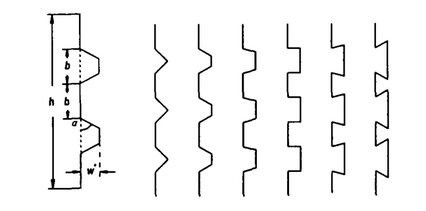
\includegraphics[width=3.4in]{./images/efield_image2.png}
		\caption{meandered monopole antenna geometry}
		\label{fig:efield_fig2}
	\end{center}
\end{figure}

The M0 configuration has a self-resonant frequency at 80MHZ, while the M5 configuration has a self-resonant frequency at 110MHZ. For antenna represented in Fig 1, s is equal to 1cm, L is equal to 4cm, using equation (2) and (3), and the value of Lm is calculated as about 300nH, a comparison table of resonant behavior of different numbers of section is listed in figure \ref{fig:efield_fig3}.

\begin{figure}[h]
	\begin{center}
		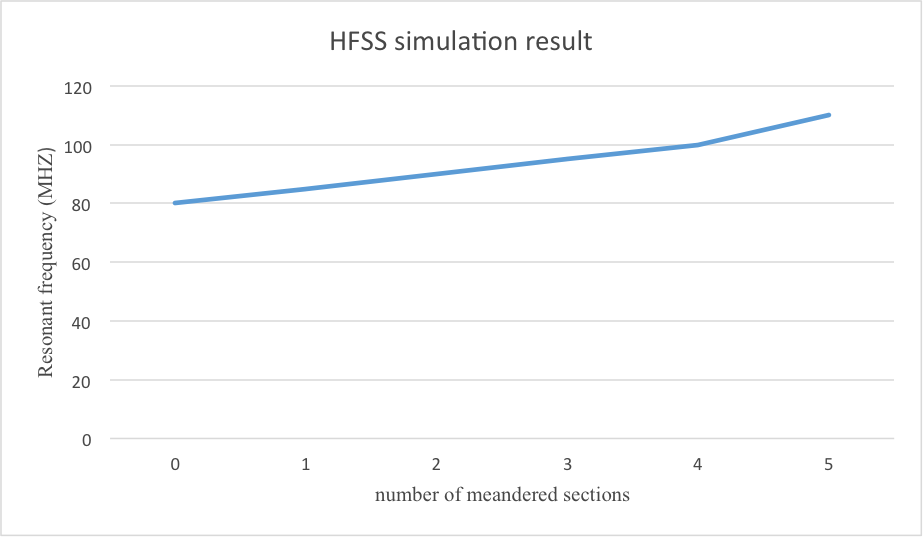
\includegraphics[width=4.3in]{./images/SG_fig3.png}
		\caption{Resonant frequency of meandered line antenna M0 to M5}
		\label{fig:efield_fig3}
	\end{center}
\end{figure}

From figure \ref{fig:efield_fig3}, it is evident that the inductor circuit model representing the meandered antenna provides an acceptable prediction showing a liner increase in resonant frequency as a function of increasing bending sections, however, in the real case, the resonant frequency of the meander line antenna will not linearly increase with the number of sections.[1],[2]

The limitation of inductor circuit model of the meandered antenna is still in examining, we simulated that some of the physical properties varied and the corresponding change of the resonant frequency. Firstly, we change the s in M1 configuration from 1cm to 2cm, the resonant frequency behavior of the antenna versus the meandered sections is shown in figure \ref{fig:efield_fig4}. We can observe that the actual resonant frequency will not precisely change as we seen in figure \ref{fig:efield_fig3}. 

\begin{figure}[h]
	\begin{center}
		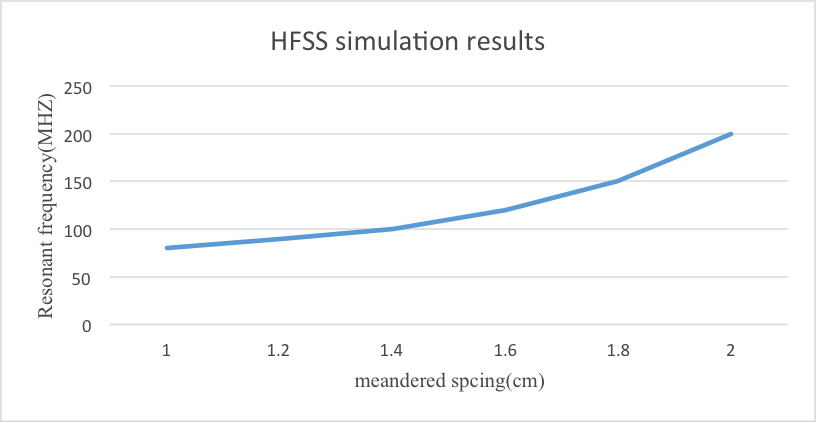
\includegraphics[width=4.3in]{./images/SG_fig4.png}
		\caption{resonant frequency vs meandered spacing}
		\label{fig:efield_fig4}
	\end{center}
\end{figure}

Next, we examined the effect of bending angle changing for each meandered section shown in figure \ref{fig:efield_fig5} [1]

\begin{figure}[h]
	\begin{center}
		
\includegraphics[width=3in]{./images/efield_image4.png}
		\caption{Bending angle when α= 45,60,75,90,120 degree conditions}
		\label{fig:efield_fig5}
	\end{center}
\end{figure}

We bend the antenna for the configuration M5 too see the simulation results in HFSS while keep the total physical length and spacing as the same as the previous model. The relation between bending angle and self-resonant frequency is shown in figure \ref{fig:efield_fig6}.

\begin{figure}[h]
	\begin{center}
		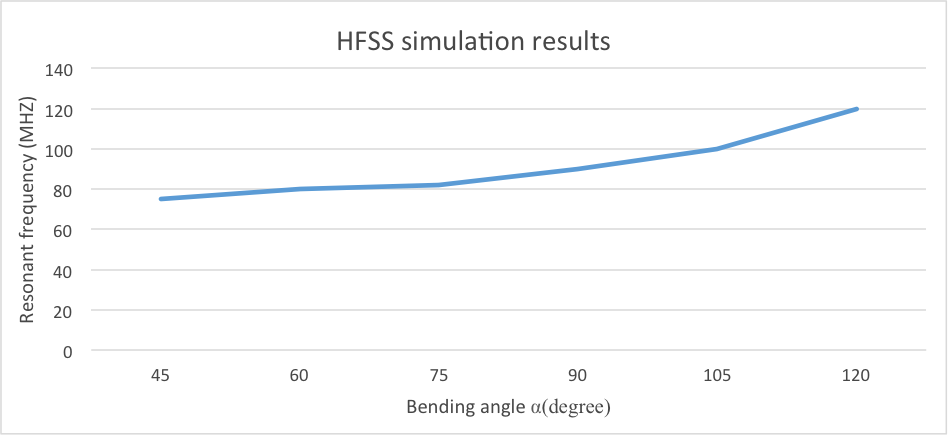
\includegraphics[width=4.3in]{./images/SG_fig5.png}
		\caption{the relation between bending angle and resonant frequency}
		\label{fig:efield_fig6}
	\end{center}
\end{figure}

It is observed that resonant frequency would experience a little fluctuate when the bending angle is changing from 45 to 120 degrees. Nevertheless, we need to obtain a relatively large difference between cross-plane and co-plane polarization, as we can see in Fig.6, the 90 degree bending angle will provide a cancellation of radiation in horizontal axis due to the opposite flowing direction of two current. At the same time, the radiation current will always along a same direction in vertical axis, as a result, the radiation of the 90 degree bending antenna is equivalent to a single line monopole antenna. Furthermore, the 90 degrees bending method will save room on PCB board so that the total physical length of the antenna will get dropped.

\begin{figure}[h]
	\begin{center}
		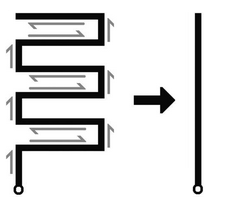
\includegraphics[width=2in]{./images/efield_image5.png}
		\caption{the relation between bending angle and resonant frequency}
		\label{fig:efield_fig7}
	\end{center}
\end{figure}

\subsection{Antenna Building and Testing}

After investigating the effects of numbers of section, section spacing and bending angle, we start to build a meandered antenna on the substrate to satisfy the specification of the antenna parameters. As seen in figure \ref{fig:efield_fig8}, the spacing between each meandered section is 0.5cm, the number of meandered sections is 14 in total, and the s11 graph is shown in figure \ref{fig:efield_fig9} which provide us a return loss below -10dB.

\begin{figure}[h]
	\begin{center}
		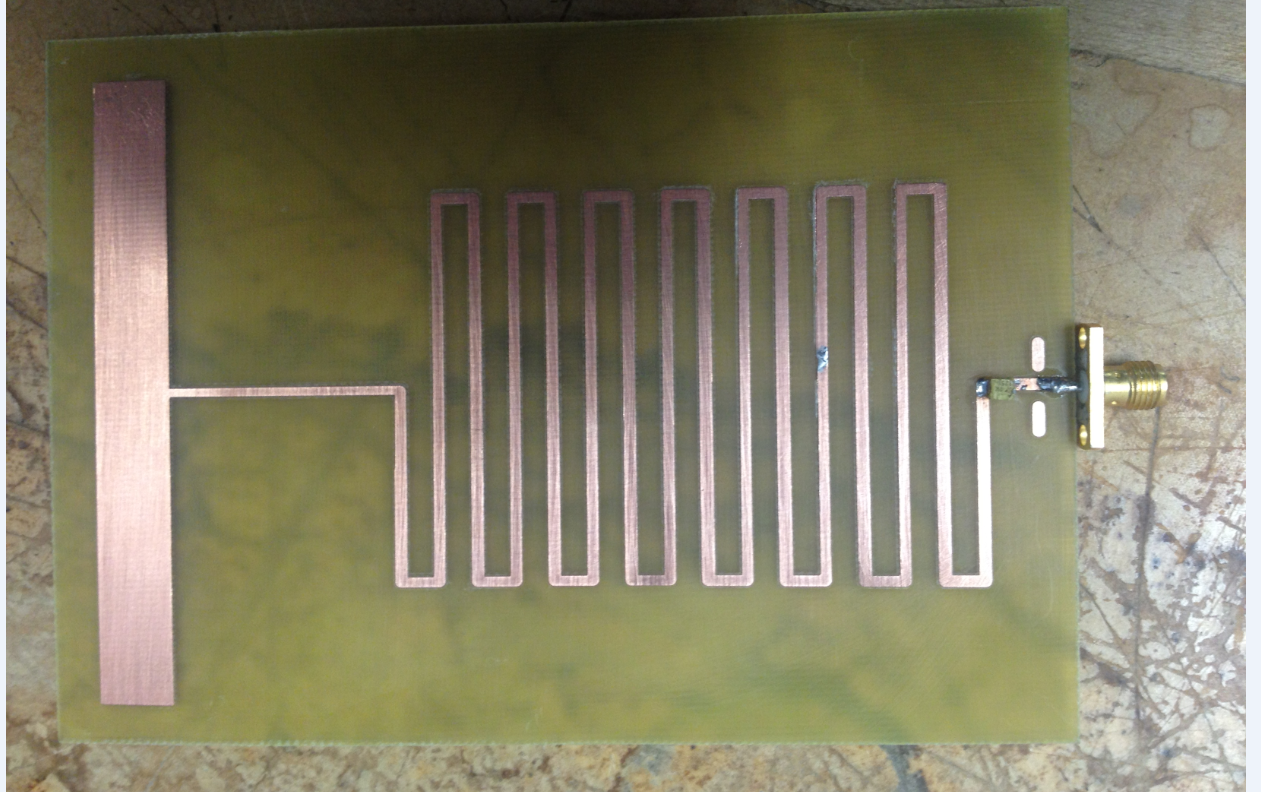
\includegraphics[width=4in]{./images/efield_image6.png}
		\caption{final antenna view}
		\label{fig:efield_fig8}
	\end{center}
\end{figure}

The physical length of this antenna is 80cm in total with the height of 10cm on the substrate, a top loading cap is added at the far end of the antenna to increase the s11 performance. To match up the resonant circuit, we add a 400nH inductor at the feeding point of the antenna. When testing the S12 parameter, we used a $\lambda/4$ dipole antenna as port 2 in HFSS so that the designed antenna is acting as a receiving antenna in the air box. The simulation model is shown in figure \ref{fig:efield_fig9}. And the simulation results are listed in figures \ref{fig:efield_fig10}, \ref{fig:efield_fig11} and \ref{fig:efield_fig12}.

\begin{figure}[h]
	\begin{center}
		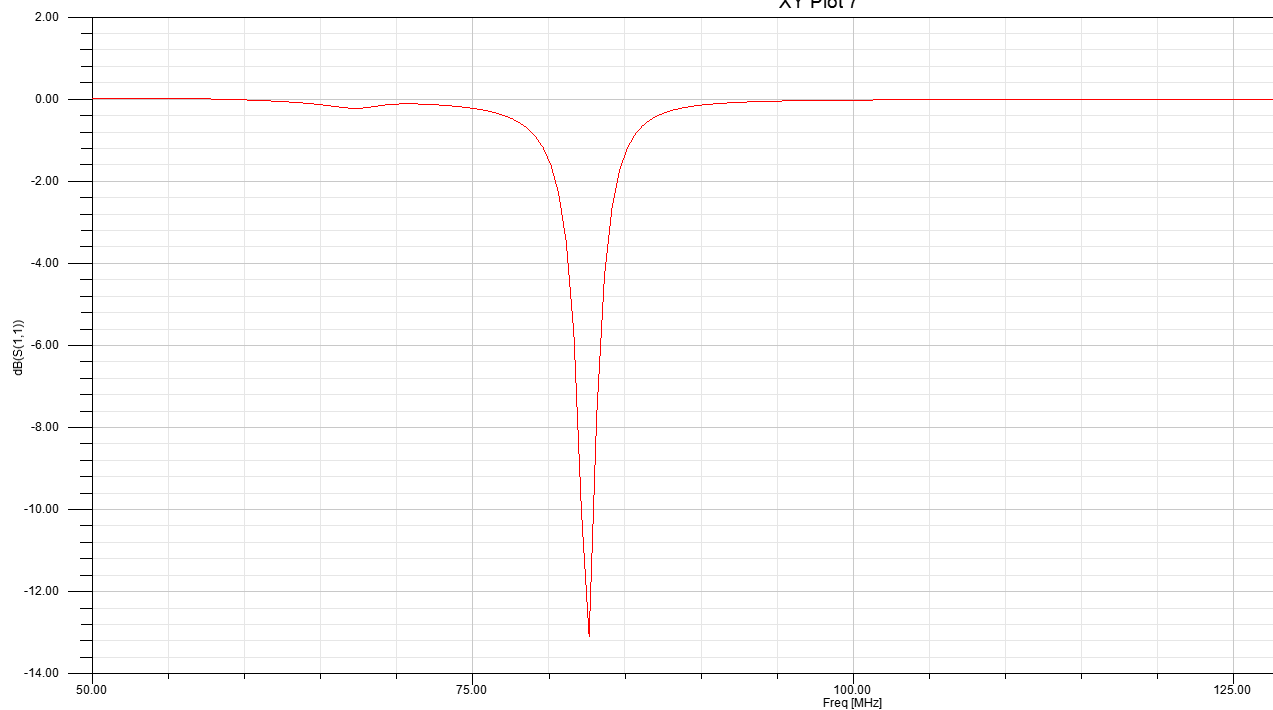
\includegraphics[width=4.3in]{./images/efield_image7.png}
		\caption{S11 curve for meandered antenna in HFSS}
		\label{fig:efield_fig9}
	\end{center}
\end{figure}

\begin{figure}[h]
	\begin{center}
		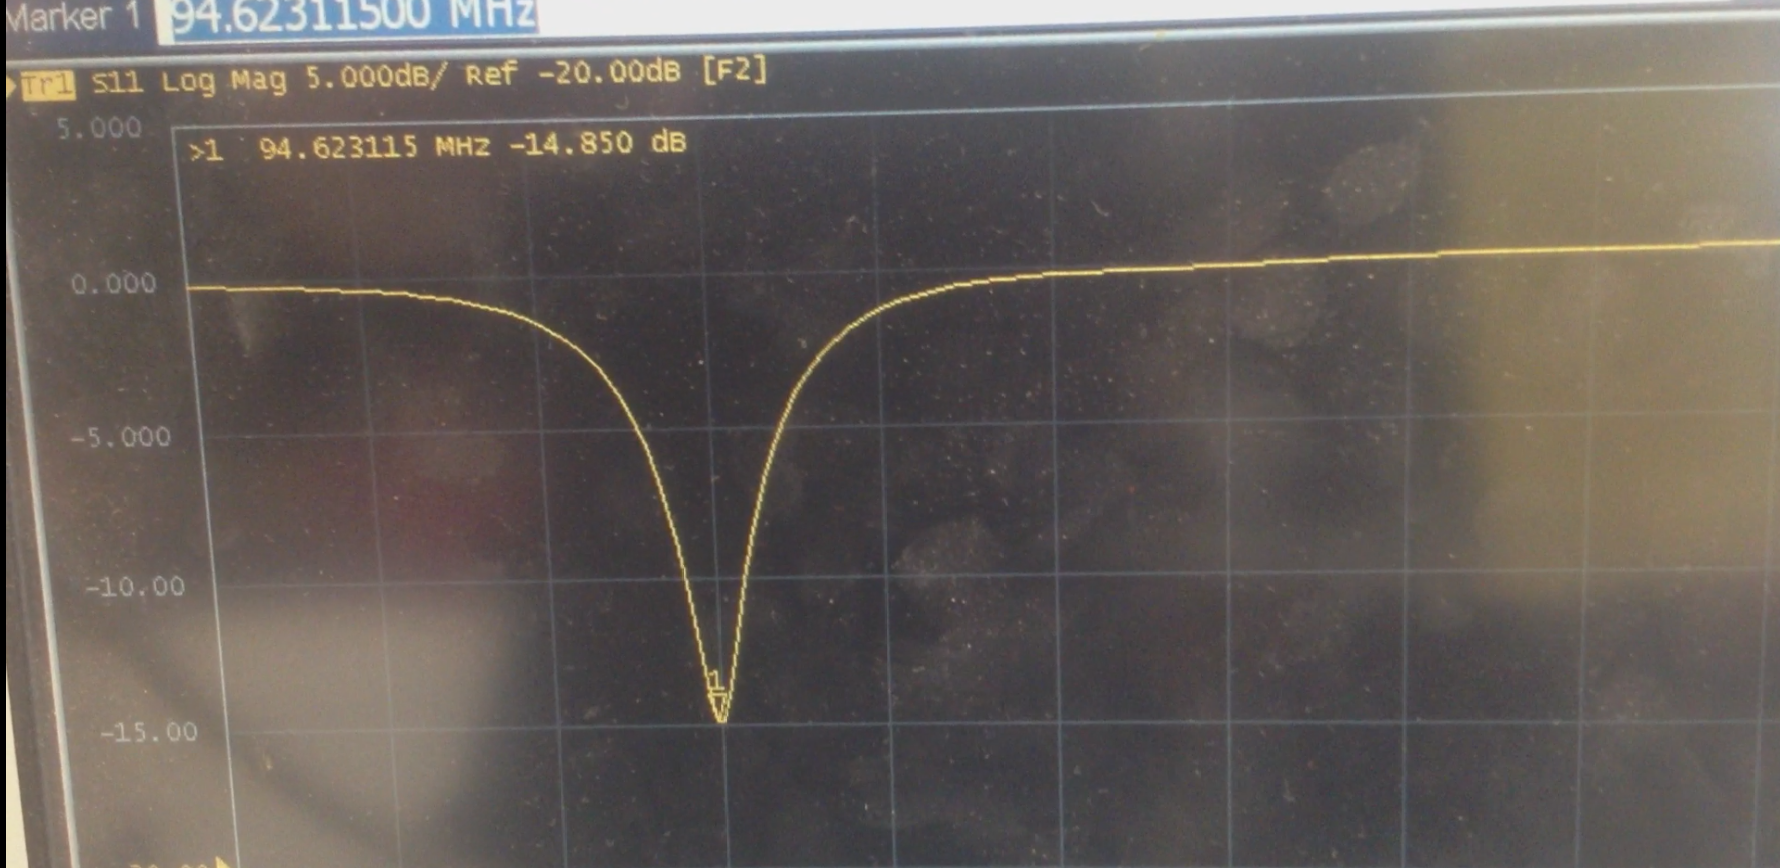
\includegraphics[width=4.3in]{./images/efield_image8.png}
		\caption{ S11 curve for real testing results}
		\label{fig:efield_fig10}
	\end{center}
\end{figure}

In the real testing, the resonant frequency got shifted to 95MHZ due to the inaccurate selection of the inductor value, since we can only get 330nH or 470nH one from the lab, the result frequency will not located in 80MHZ.

\begin{figure}[h]
	\begin{center}
		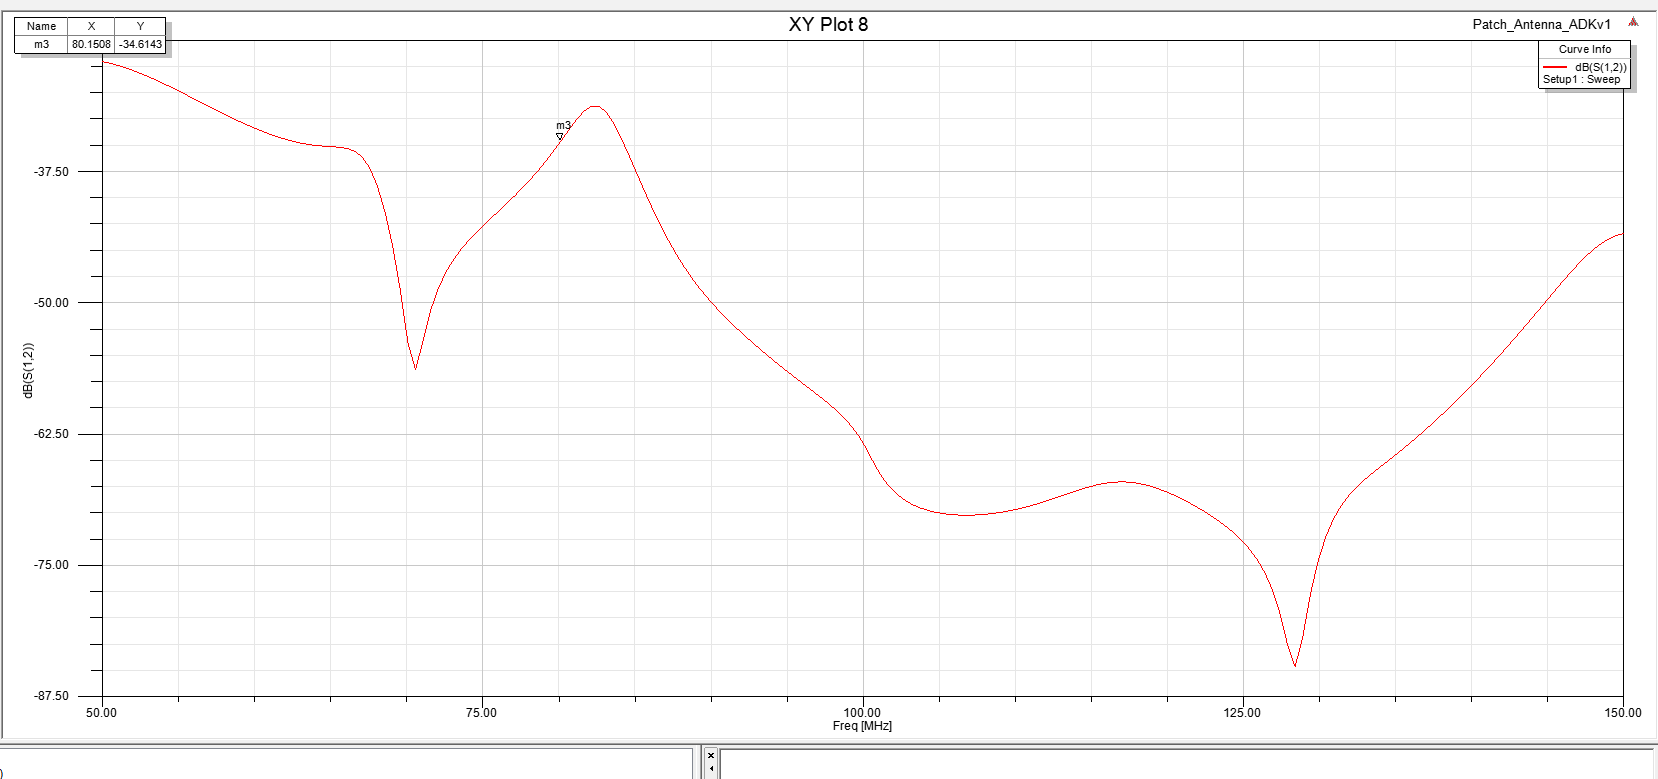
\includegraphics[width=4.7in]{./images/efield_image9.png}
		\caption{ S12 curve for cross-plane polarization in HFSS}
		\label{fig:efield_fig11}
	\end{center}
\end{figure}

\begin{figure}[h]
	\begin{center}
		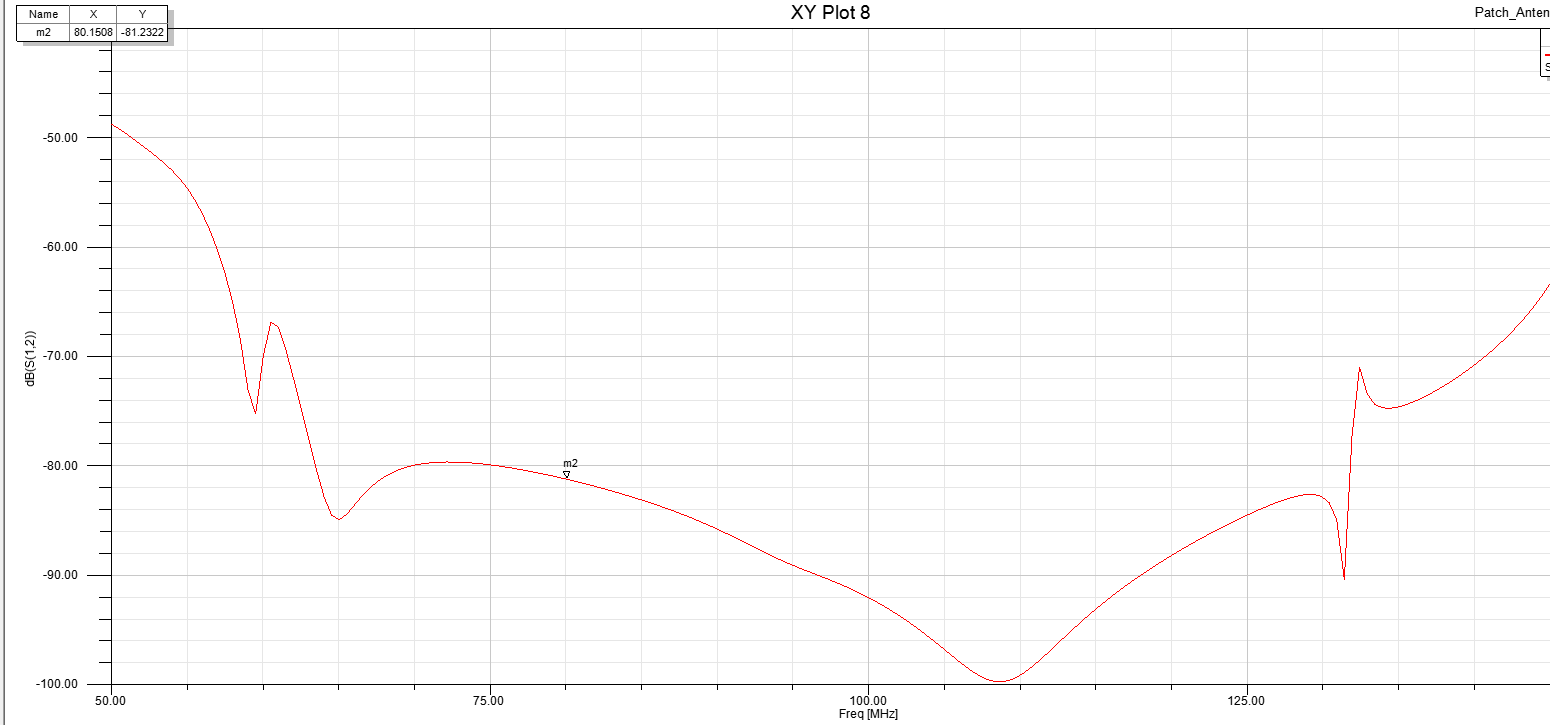
\includegraphics[width=4.7in]{./images/efield_image10.png}
		\caption{S12 curve for co-plane polarization in HFSS}
		\label{fig:efield_fig12}
	\end{center}
\end{figure}

\clearpage

\begin{figure}[h]
	\begin{center}
		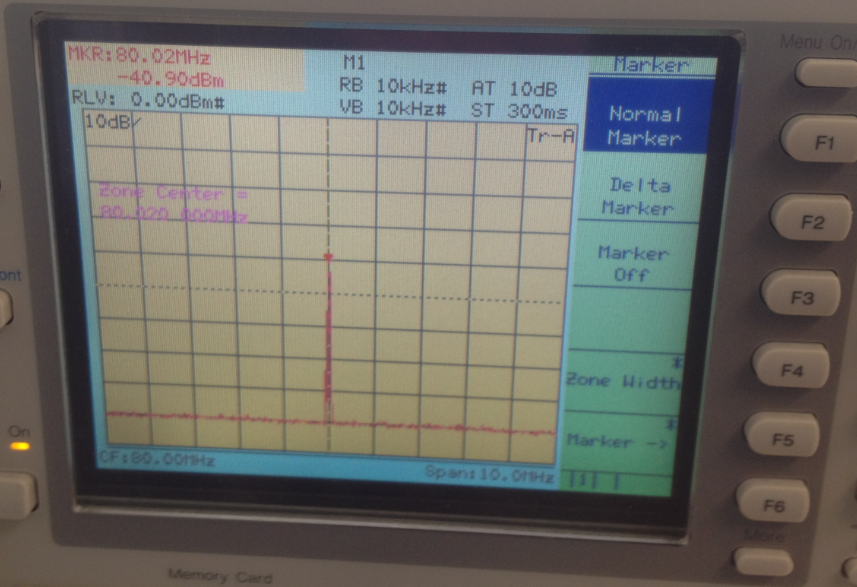
\includegraphics[width=3.4in]{./images/efield_image11.png}
		\caption{S12 curve for cross-plane polarization in real test}
		\label{fig:efield_fig13}
	\end{center}
\end{figure}

\begin{figure}[h]
	\begin{center}
		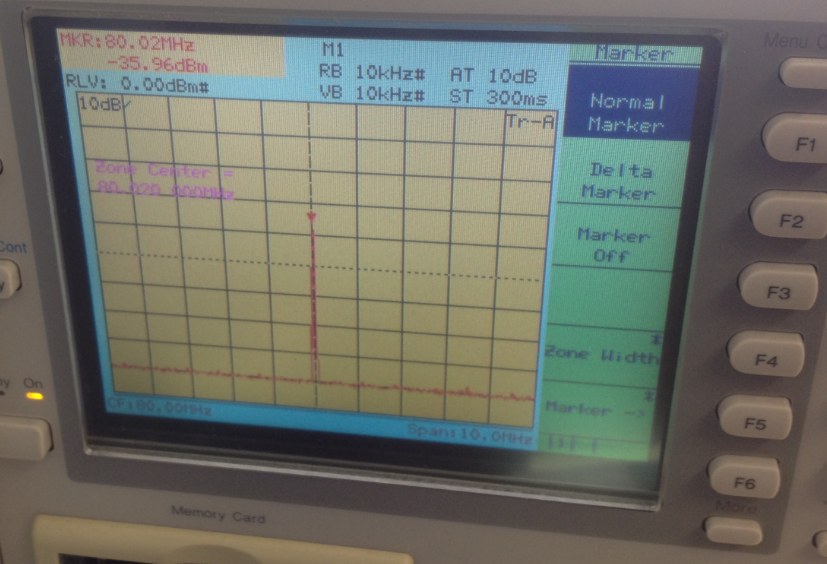
\includegraphics[width=3.4in]{./images/efield_image12.png}
		\caption{S12 curve for co-plane polarization in real test}
		\label{fig:efield_fig14}
	\end{center}
\end{figure}

\clearpage

As a conclusion, for s12 curves, in HFSS the results is pretty good that difference between co-plane and cross-plane of s12 is about 15dB, but in the real test, the difference is 5db, the cause for the difference in quantity is from the non-ideal air box and ground plane from the lab comparing to the ideal ones in HFSS. Further improvement for the testing method is still required.




	%!TEX root =  ../final-report.tex

% Chapters are setup to start on a new page.
% The short version of that title appears in square brackets. This is used for the table of contents listing. 
% The long version of the title has a command "\setstretch{0.5}" in order to reduce the line spacing in the
% title and then the title text.

\section{H-field Antenna}

\subsection{Purpose}

Normally microwave imaging systems consist of a simple E-field antenna such and a Monopole or a Dipole antenna which has one polarization and it is limited in its functionality, however it is simple to model in the imaging inversion algorithm as these types of antennas have very simple and well defined current distributions along them. Due to a grain storage bin being round, metallic, and closed off at both ends, it can be thought of as a cylindrical resonant chamber which introduces a level of difficulty in designing antennas that can operate in such an environment. However since the walls of the bin are metallic, the field components at the metallic walls are easily differentiable, the H-fields are tangential to the metallic walls of the chamber, and the E-fields are perpendicular to the walls, thus we would like to have an antenna that is capable of probing the tangential H-fields only.

The H- field antenna design had to be confined to the following design criteria in order for it to be effective inside of the grain bin:

\begin{itemize*}

\item Ability to pick up H-field only, and reject most of the E-field
\item Minimal size (less that 15cm in length or witdth)ˆ
\item Frequency of operation between 70Mhz-90Mhzˆ
\item Matched to 50 ohm coaxial transmission lineˆ
\item Physically able to withstand grain being filled into the binˆ
\item Reduced complexity(for ease of modeling in the inversion algorithm)ˆ
\item Ease of manufacturing and reproduction

\end{itemize*}

\subsection{Research}

The typical design procedure for an H-field antenna is a loop of perimeter one $\lambda$ as at that length the loop becomes purely resistive with the maximum amount of radiation resistance, however this approach does not work for the grain bin as the perimeter of the loop would have to be almost 4 meters.

The other typical approach to designing h-field antennas is to decrease the perimeter of the loop and increase the number of turns which allows for the required size reduction that we are looking for as well as enable it to be matched to a 50ohm coaxial line since the radiation resistance is proportional to the number of turns squared $R_r = (\frac{177NS}{\lambda})^2$, however it is also not feasible for the grain bin since it would not guarantee that the antenna does not pick up the E-field as well, and it would be too complex to model in the imaging software.

\subsection{Design}

In order to satisfy the main requirement of the antenna (1) a shielded and slotted loop antenna was chosen, which is a common type of antenna used in radio.

\begin{figure}[h]
	\begin{center}
		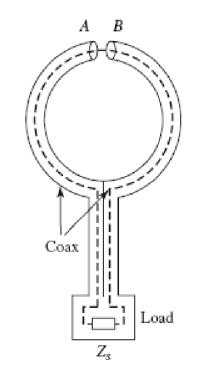
\includegraphics[width=1.5in]{./images/Figure1.jpg}
		\caption{}
		\label{fig:hfield_fig1}
	\end{center}
\end{figure}

The ground layer around the conductor which acts as the shielding modifies the electric field distribution inside of the antennas cross sectional area due to the boundary conditions on a PEC, thus reducing its effect on the antenna, this effect is confirmed in the simulation results in section \ref{sec:sim_results}. Since the magnetic field passing through the loop induces a current on both the conductor and the shielding, a slot is cut out in the shield to create a capacitance which introduces a phase shift between the two currents and therefore there is a difference in potential across the load.

The second requirement (2) was met by reducing the perimeter of the antenna to $\lambda /20$, however the small size presented another challenge which is matching the loop antenna to the 50ohm coaxial line, different ways of matching were considered such as capacitive coupling and transformer coupling between the coaxial line and the antenna, These were simulated in HFSS but found the it would be too complex to build accurately, and it would not be feasible to mount in the grain bin. Mohammad (Project co-supervisor) suggested the use of a 50ohm termination at the end of the loop to match the antenna to a 50ohm line and to cut the loop in half so that the size of it could be further reduced as well as to take advantage of having a metallic wall as the other half of the loop. A prototype of this antenna was built using a semi rigid coaxial cable with a slot cut in the ground conductor and a 50 ohm termination was used to match the antenna to a coaxial line.

\begin{figure}[h]
	\begin{center}
		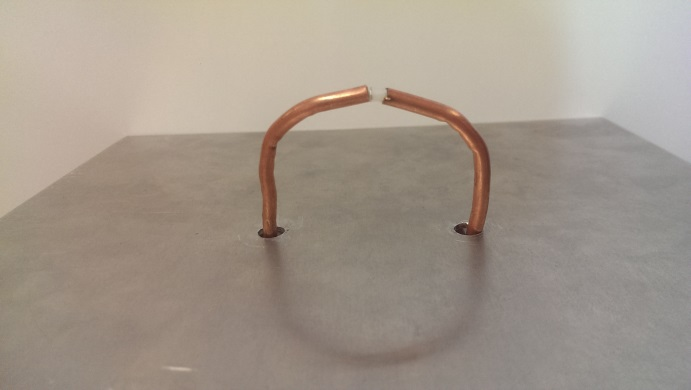
\includegraphics[width=4in]{./images/Figure2.jpg}
		\caption{prototype antenna}
		\label{fig:hfield_fig2}
	\end{center}
\end{figure}

A difference of 10db was observed between the E and H polarization. However building multiples of such antennas accurately would not be feasible since the slot size would vary and produce inaccurate results as well as the curvature in the antenna is tough to reproduce accurately.

In order to make the antenna easy to manufacture and reproduce, it was decided that a PCB version would be best suitable.

\subsection{PCB Antenna Design}

To achieve a shielded coaxial line on PCB, a groundless co-planar waveguide was chosen, due to material availability, 0.8mm FR-4 material was chosen as the PCB material with a relative permittivity of 4.3. Due to the limited capabilities of the PCB prototyping machine available at the EIL lab, a minimum cut in the PCB could not exceed 0.2mm, therefore 0.2mm was chosen as the gap between the conductor and the ground planes of the co-planar waveguide. With the help of TX-line (transmission line calculation software) a conductor size of 2.57mm with a gap of 0.2mm and a 0.8mm FR-4 thickness yields the necessary 50ohm transmission line. The size of the antenna is 12.5cm in length and 5.5cm in width with 45 degree bends for reducing reflections, the bent sections are 1cm long.

\subsection{PCB Antenna Simulation}

The PCB version of the antenna is constructed in the high frequency structure simulator with FR-4 as the substrate material, copper material on top of the substrate is simulated as perfect conductor and an infinite ground plane as the antennas backing plate. The design is simulated and optimized to obtain its performance characteristics. From optimization a slot size of 1 mm is chosen in the shielding.

\begin{figure}[h]
	\begin{center}
		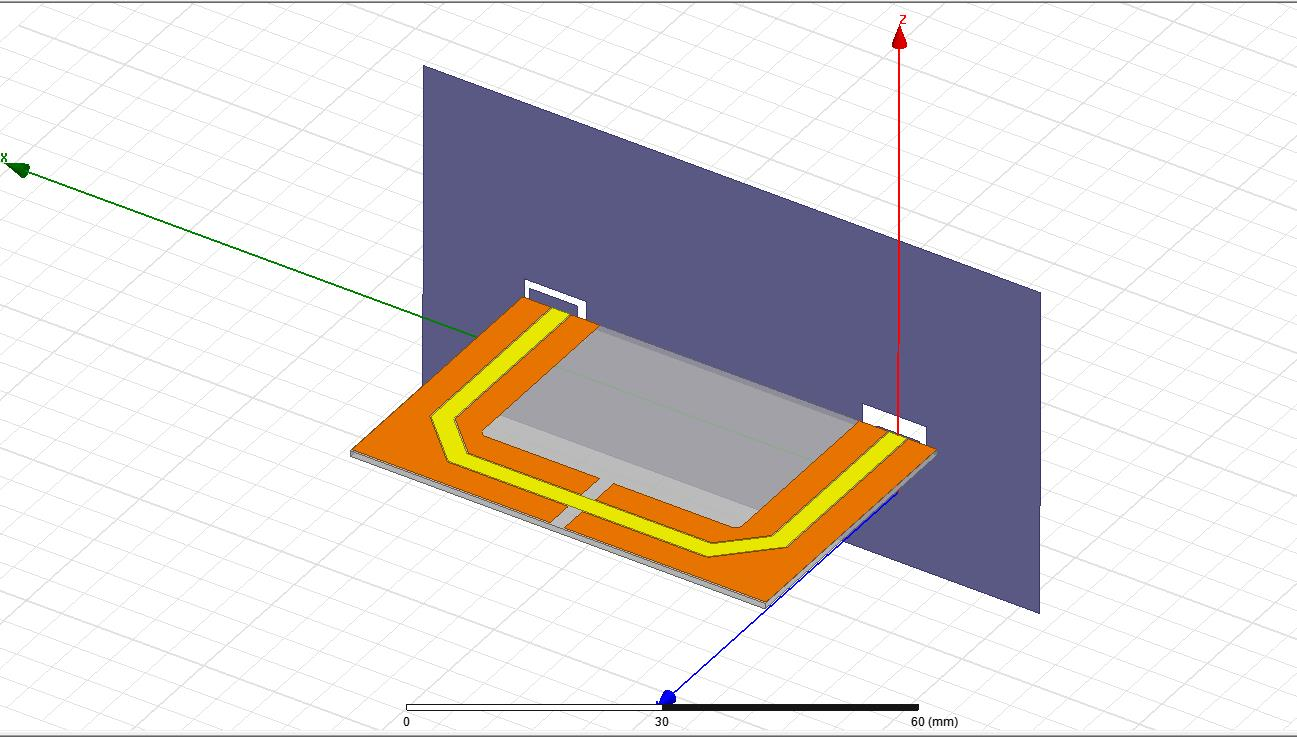
\includegraphics[width=4in]{./images/Figure3.jpg}
		\caption{HFSS model}
		\label{fig:hfield_fig3}
	\end{center}
\end{figure}

\subsection{Simulation Results}
\label{sec:sim_results}

The desired result is to have an S11 (insertion loss) of -10db at the frequency of operation, and as expected the insertion loss at 80 MHz is -14.5db as well as due to the 50 ohm termination the antenna has a really high bandwidth.

The simulation also confirms the effect of the co-planar ground plane on the Electric fields inside the cross sectional area of the antenna, Figure 6 and Figure 7 show the antenna with shielding and antenna without shielding E-field magnitude distribution in the cross sectional area.

\begin{figure}[h]
	\begin{center}
		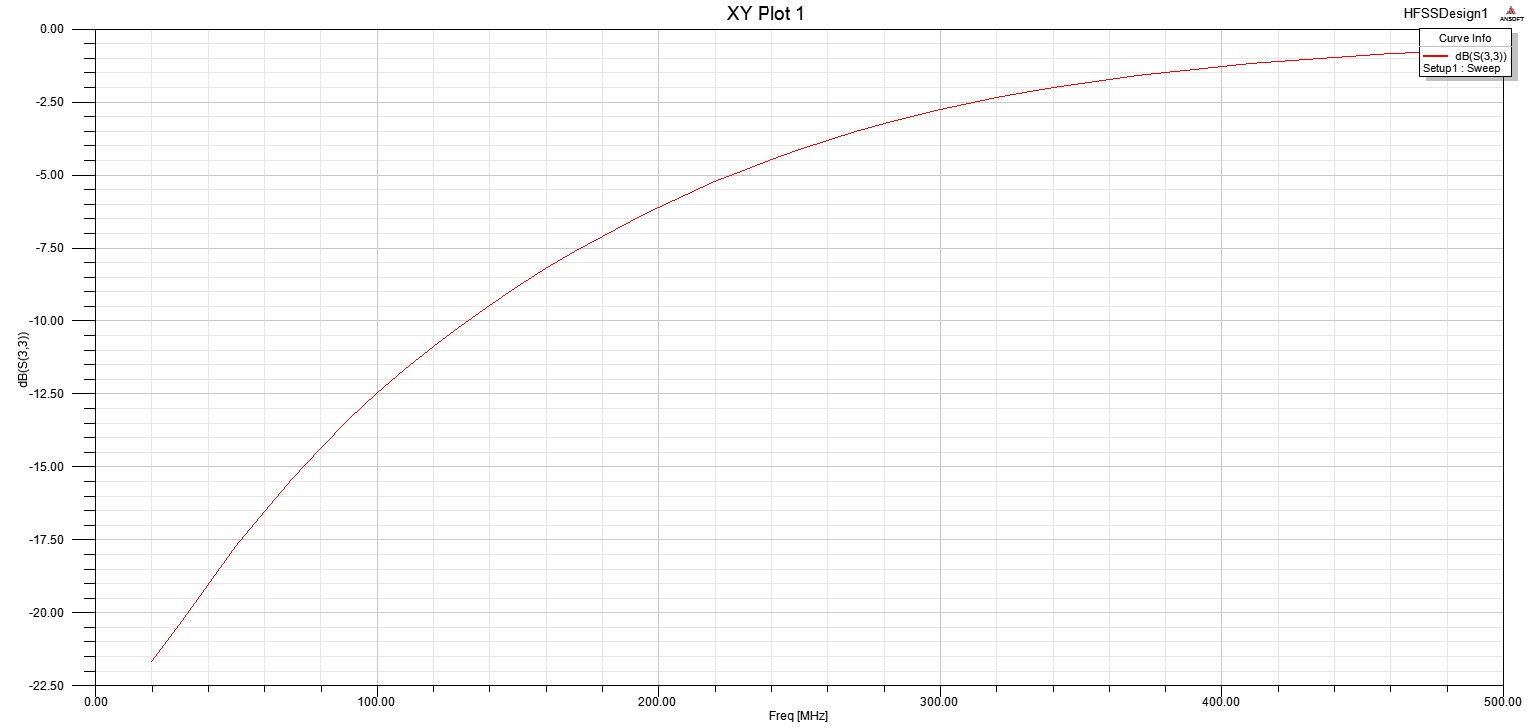
\includegraphics[width=5in]{./images/Figure4.jpg}
		\caption{S11}
		\label{fig:hfield_fig4}
	\end{center}
\end{figure}

\begin{figure}[h]
	\begin{center}
		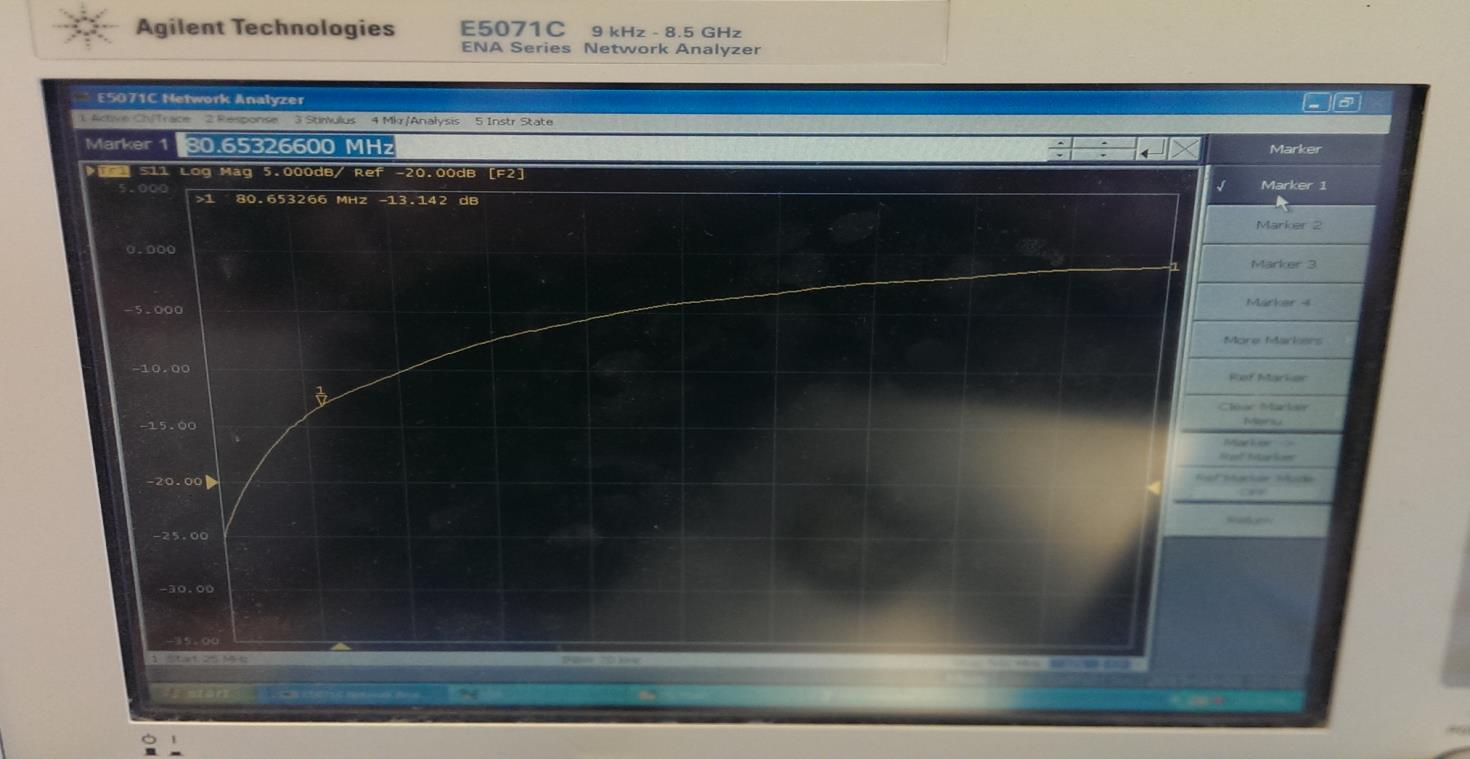
\includegraphics[width=5in]{./images/Figure5.jpg}
		\caption{Built antenna S11}
		\label{fig:hfield_fig5}
	\end{center}
\end{figure}

\begin{figure}[h]
	\begin{center}
		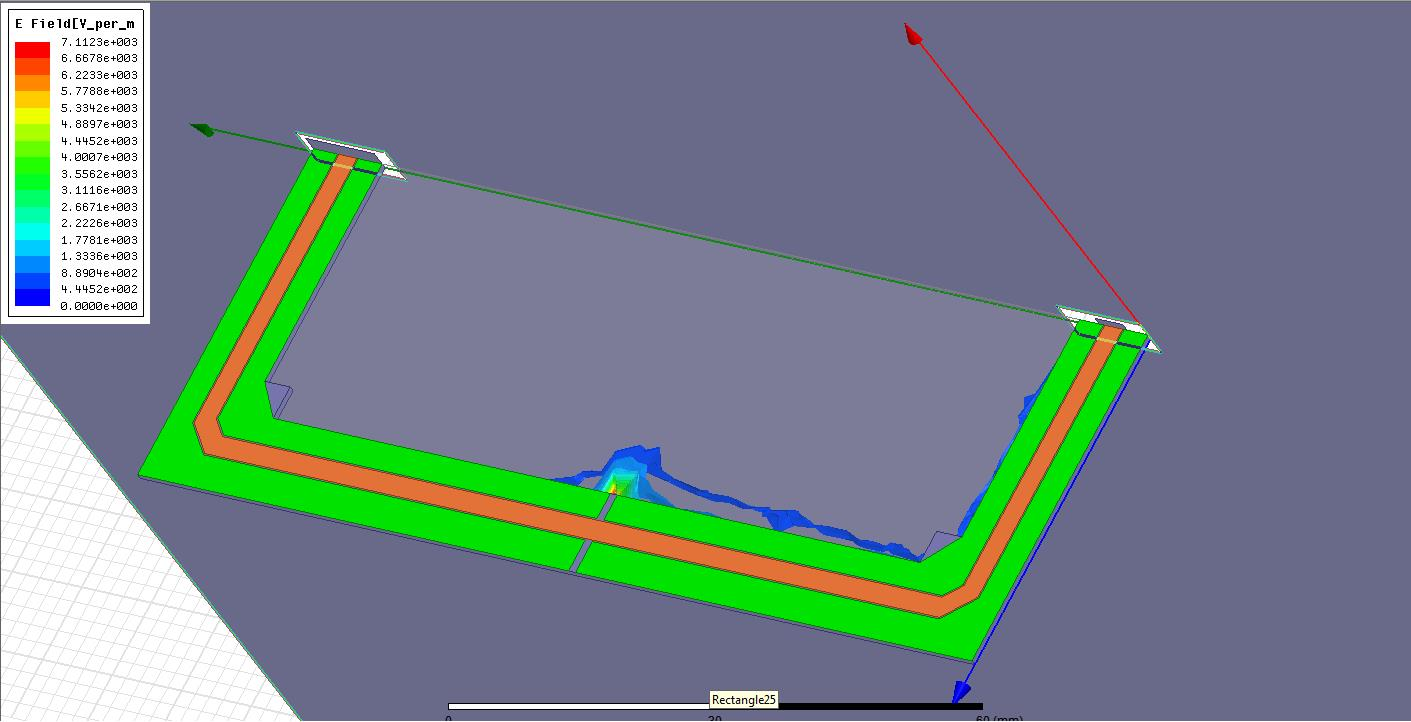
\includegraphics[width=4in]{./images/Figure6.jpg}
		\caption{Loop antenna with shielding}
		\label{fig:hfield_fig6}
	\end{center}
\end{figure}

\begin{figure}[h]
	\begin{center}
		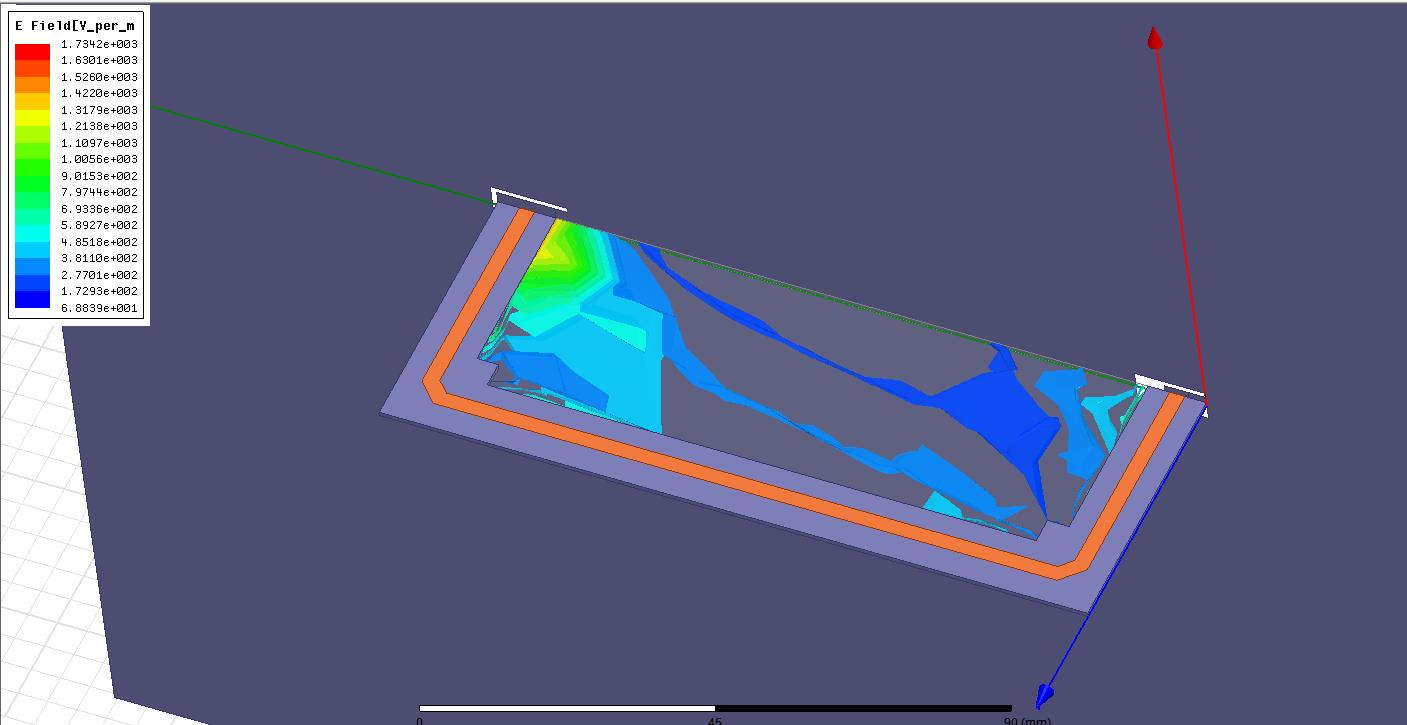
\includegraphics[width=4in]{./images/Figure7.jpg}
		\caption{Shielding removed}
		\label{fig:hfield_fig7}
	\end{center}
\end{figure}

\subsection{PCB Layout}

After simulating the antenna in HFSS, the design was transferred to Altium which was used to create the necessary Gerber files for fabrication. The antenna was fabricated in the EIL with the use of the rapid PCB prototyping machine.

\begin{figure}[h]
	\begin{center}
		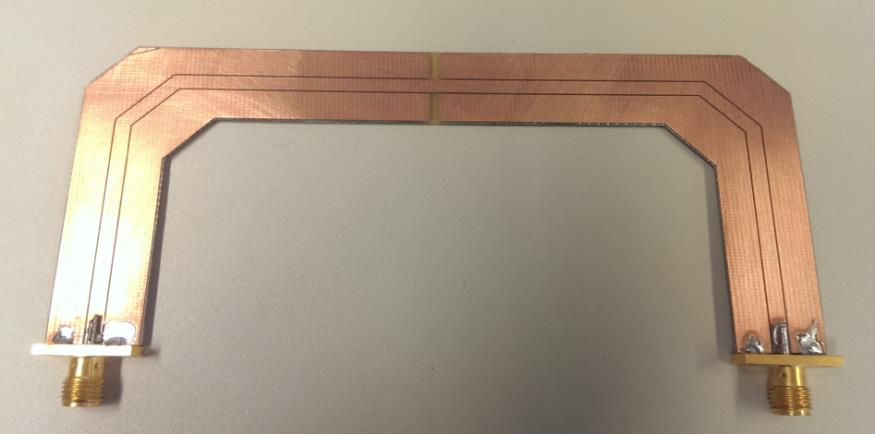
\includegraphics[width=4in]{./images/Figure8.jpg}
		\caption{fabricated antenna}
		\label{fig:hfield_fig8}
	\end{center}
\end{figure}

\subsection{H-field Antenna Testing}

The antenna’s ability to reject the Electric field was tested in a G-TEM cell. The G-TEM cell creates transverse EM waves guided between a pair of plates with H orthogonal to E, the incident wave was created with a signal generator producing an 80 MHz sine wave with 0dbm power and the AUT measurements were taken with a spectrum analyzer. Two orientations of the antenna were tested in the cell, longitudinally parallel with the magnetic field (E-orientation) and perpendicular to magnetic field (H-orientation).

\begin{figure}[h]
	\begin{center}
		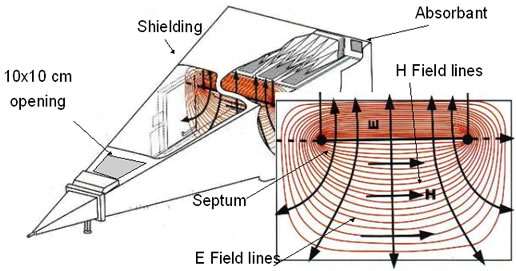
\includegraphics[width=4in]{./images/image9.jpeg}
		\caption{field lines in G-TEM for reference}
		\label{fig:hfield_fig9}
	\end{center}
\end{figure}

\subsection{G-TEM Test Results}

The noise floor of the antenna was measured at -83dbm with incident power of -13dbm.

When oriented in the E-orientation the antenna received -81dbm which is close to the noise level of the antenna, when oriented in the H-orientation the antenna received -65dbm therefore a difference of 16db exists between the two orientations which shows that the antenna is picking up only H-field.

\begin{figure}[h]
	\begin{center}
		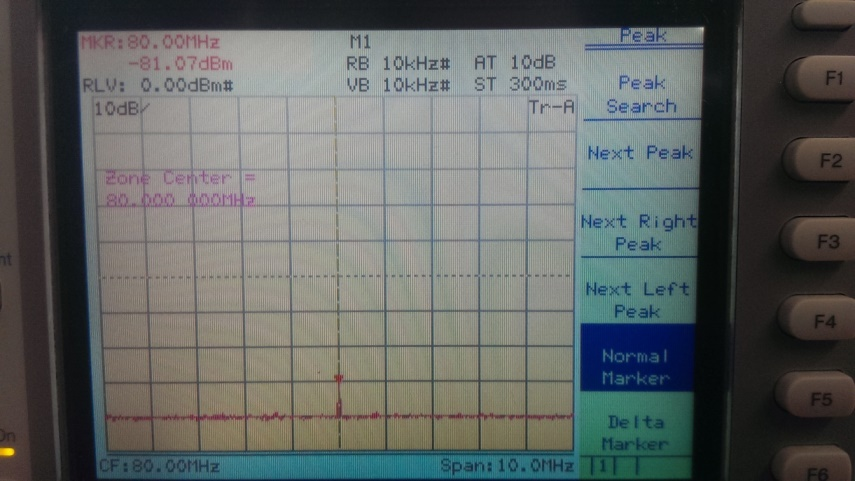
\includegraphics[width=4in]{./images/Figure9.jpg}
		\caption{E-orientation}
		\label{fig:hfield_fig10}
	\end{center}
\end{figure}

\begin{figure}[h]
	\begin{center}
		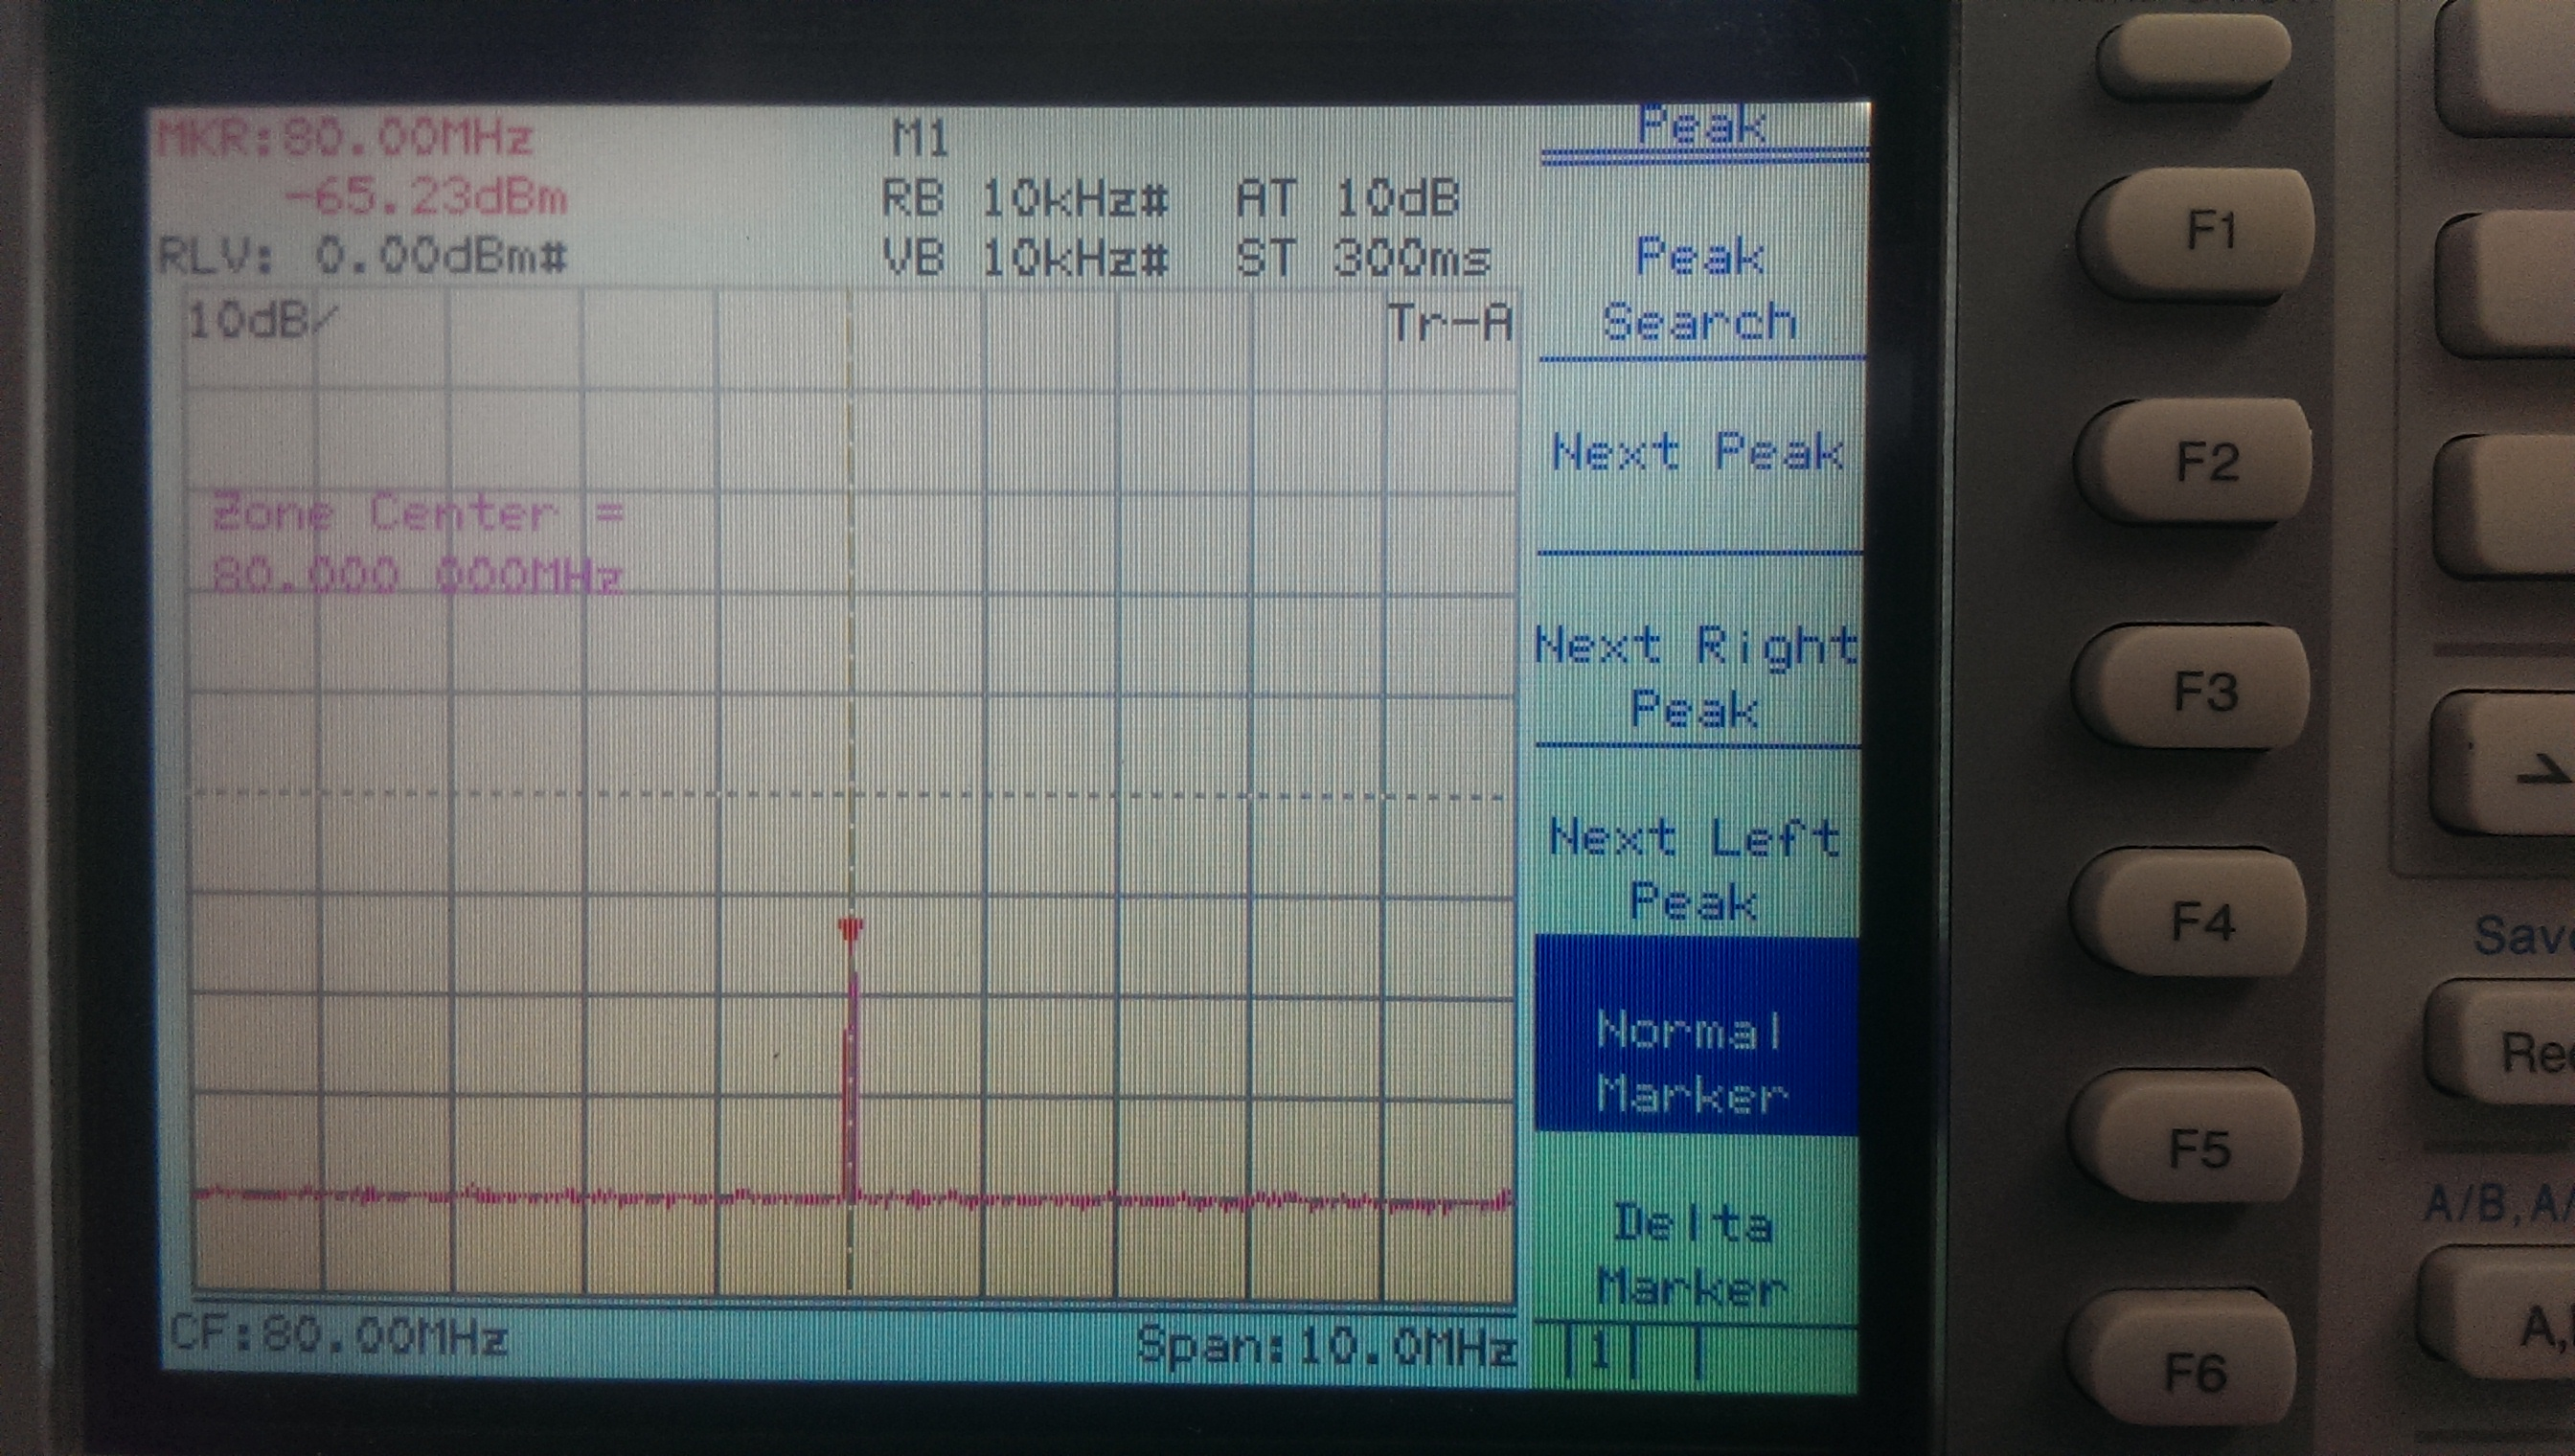
\includegraphics[width=4in]{./images/Figure10.jpg}
		\caption{H-orientation}
		\label{fig:hfield_fig11}
	\end{center}
\end{figure}


	%!TEX root =  ../final-report.tex

% Chapters are setup to start on a new page.
% The short version of that title appears in square brackets. This is used for the table of contents listing. 
% The long version of the title has a command "\setstretch{0.5}" in order to reduce the line spacing in the
% title and then the title text.

\chapter{Multiplexer}
\label{sec:Multiplexer}

The multiplexer consists of two sections; an RF switch section and a DC switch section. The RF switch provides a path for the signal to and from the VNA to the antennas, while the DC switch provides the logic necessary to set the correct path in the RF switch at the correct time. In order to collect the data required to create an image of the grain bins contents, an array of antennas needs to be connected to the VNA. Figure \ref{fig:mp_connections} shows how the multiplexer connects the VNA to the array of antennas. The VNA has two ports, one which transmits a signal and one which receives a signal. Through commands sent from the DC switch, the multiplexer is capable of connecting either of these two ports to any of the antennas in the array.

\section{RF Switch}

\subsection{Background}

The multiplexer must connect the ports from the VNA in a certain sequence. First, the multiplexer will be configured to connect the transmitter port from the VNA to antenna 1. After this, antenna 2 will be connected to the receiver port of the VNA. Then antenna 3 connects to the receiver port, then antenna 4 and so on through the entire array of antennas. Once this sequence has been completed the multiplexer will now be configured to connect the transmitter port of the VNA to antenna 2, after which antenna 1 will be connected to the receiver port, then antenna 3, then antenna 4 and so on through the entire array again. The multiplexer will repeat this sequence until all antennas have acted as the transmitter with the remaining antennas acting as receivers.

\begin{figure}[h]
	\begin{center}
		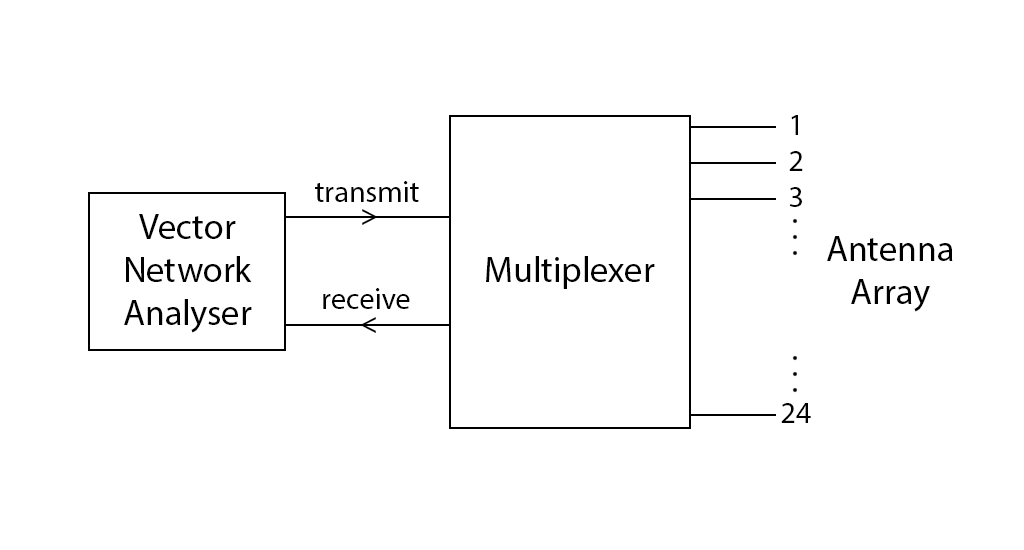
\includegraphics[width=4.5in]{./images/multiplexer_connections.png}
		\caption{Multiplexer connecting VNA to antenna array}
		\label{fig:mp_connections}
	\end{center}
\end{figure}

\subsection{Design}

An initial design for the RF multiplexer was created using six 4 x 2 matrix switches together two SP3Ts. The topology of this design is shown in figure \ref{fig:mp_initial_layout}. Note that not all of the 4 x 2 matrix switches are shown in the figure, 4 more of these switches are connected to the two remaining pins of the two SP3Ts for a total of 24 antennas. The 4 x 2 matrix switch chosen for this design was from Hittite Microwave Corporation, part number HMC596LP4 and the SP3Ts chosen were part number HMC245QS16 also from Hittite Microwave Corporation.  This design was chosen for its simplicity which would allow for good performance.

However, we were not able to use this design, as it was realized that the 4 x 2 matrix switches chosen do not operate in the frequency range needed for our project of 70 - 90 MHz. More research was done but no switches of this type were found that operate in the required frequency range for this project. Due to this limitation a new design was chosen consisting of a series of cascaded RF switches, including SPDTs, SP3Ts and SP8Ts. The topology of this design is shown in figure \ref{fig:mp_final_layout}. The switches used in this design are HMC349MS8G, HMC245QS16 and HMC253QS24 from Hittite Microwave Corporation.


\begin{figure}[h]
	\begin{center}
		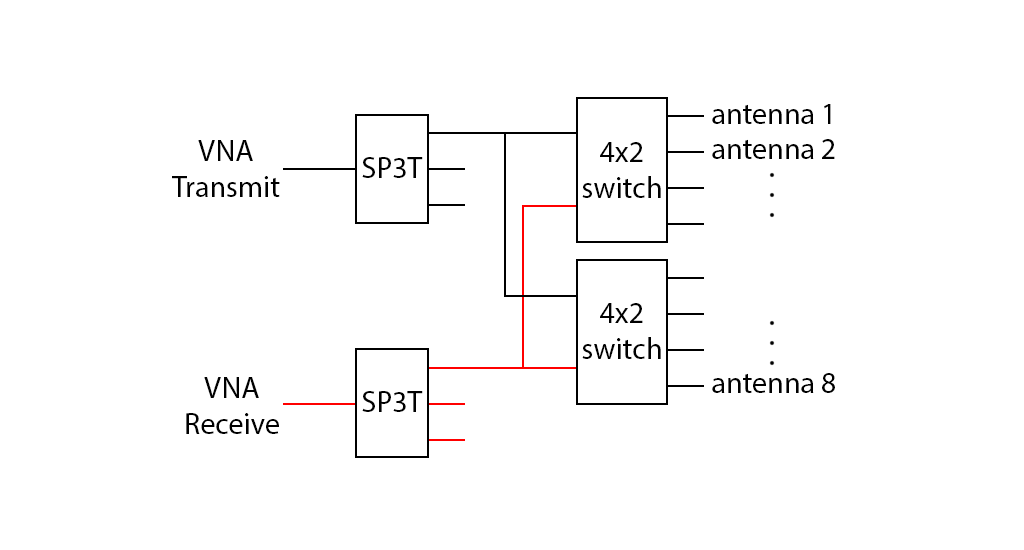
\includegraphics[width=5in]{./images/mp_initial_layout.png}
		\caption{Initial design of the multiplexer}
		\label{fig:mp_initial_layout}
	\end{center}
\end{figure}

\begin{figure}[h]
	\begin{center}
		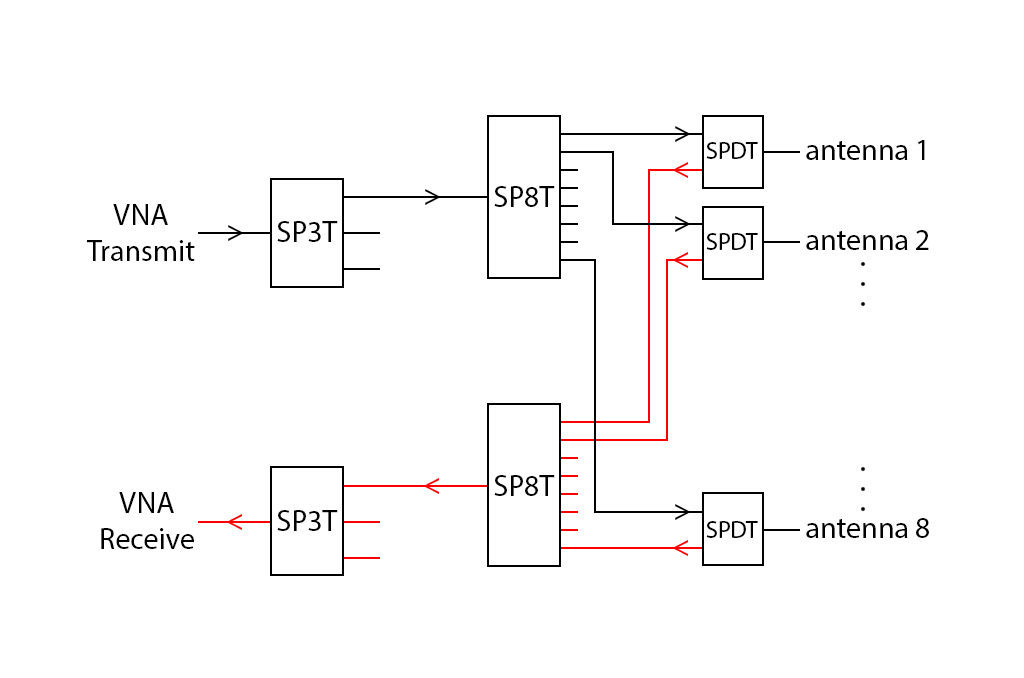
\includegraphics[width=5in]{./images/mp_final_layout.png}
		\caption{Final design of the multiplexer}
		\label{fig:mp_final_layout}
	\end{center}
\end{figure}


With this design decided on, we needed to get it manufactured on PCB. To create the PCB layout necessary to get these boards printed, software package Altium was used. Two boards were designed for the RF portion of the multiplexer; one containing only an SP3T and one containing two SP8Ts and eight SPDTs. The final 2 x 24 multiplexer requires two of the boards with SP3Ts and three of the boards with SP8Ts and SPDTs. The final PCB layout of the two boards is shown in figures \ref{fig:sp3t}, \ref{fig:sp8t_top} and \ref{fig:sp8t_bottom}.

Both boards were designed with 4 layers using a substrate of FR-4. The stack up of the boards consists of a top signal layer, followed by a substrate layer, then an internal signal layer (used only as ground in this design) and then the prepreg layer. Below the prepreg layer is a mirror of what is on top of it; an internal signal layer, then substrate layer and then bottom layer. The stack up from Altium is shown in figure \ref{fig:stackup}. 

Both boards used co-planar waveguides with ground for all of the RF traces and were designed such that they were 50 ohms. This resulted in a trace width of 0.5 mm and a gap of 0.115 mm with a substrate thickness of 0.6 mm. Three 10 pin connectors were added to provide power as well as connect all of the control pins for the SP8T and SPDT switches \cite{rob1}.

 
\begin{figure}[h]
	\begin{center}
		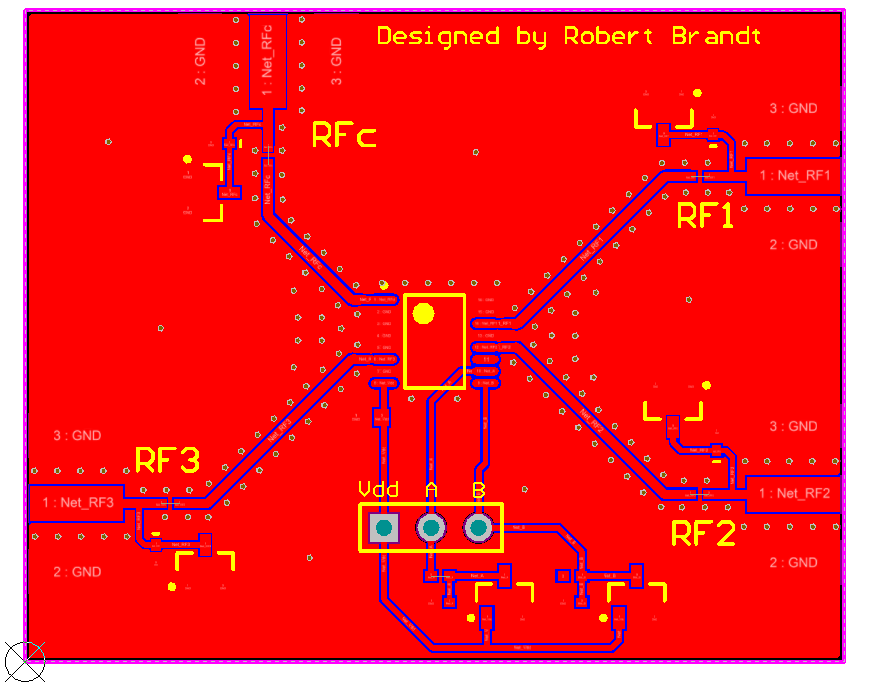
\includegraphics[width=3.5in]{./images/sp3t.png}
		\caption{PCB layout for SP3T board}
		\label{fig:sp3t}
	\end{center}
\end{figure}

\begin{figure}[h]
	\begin{center}
		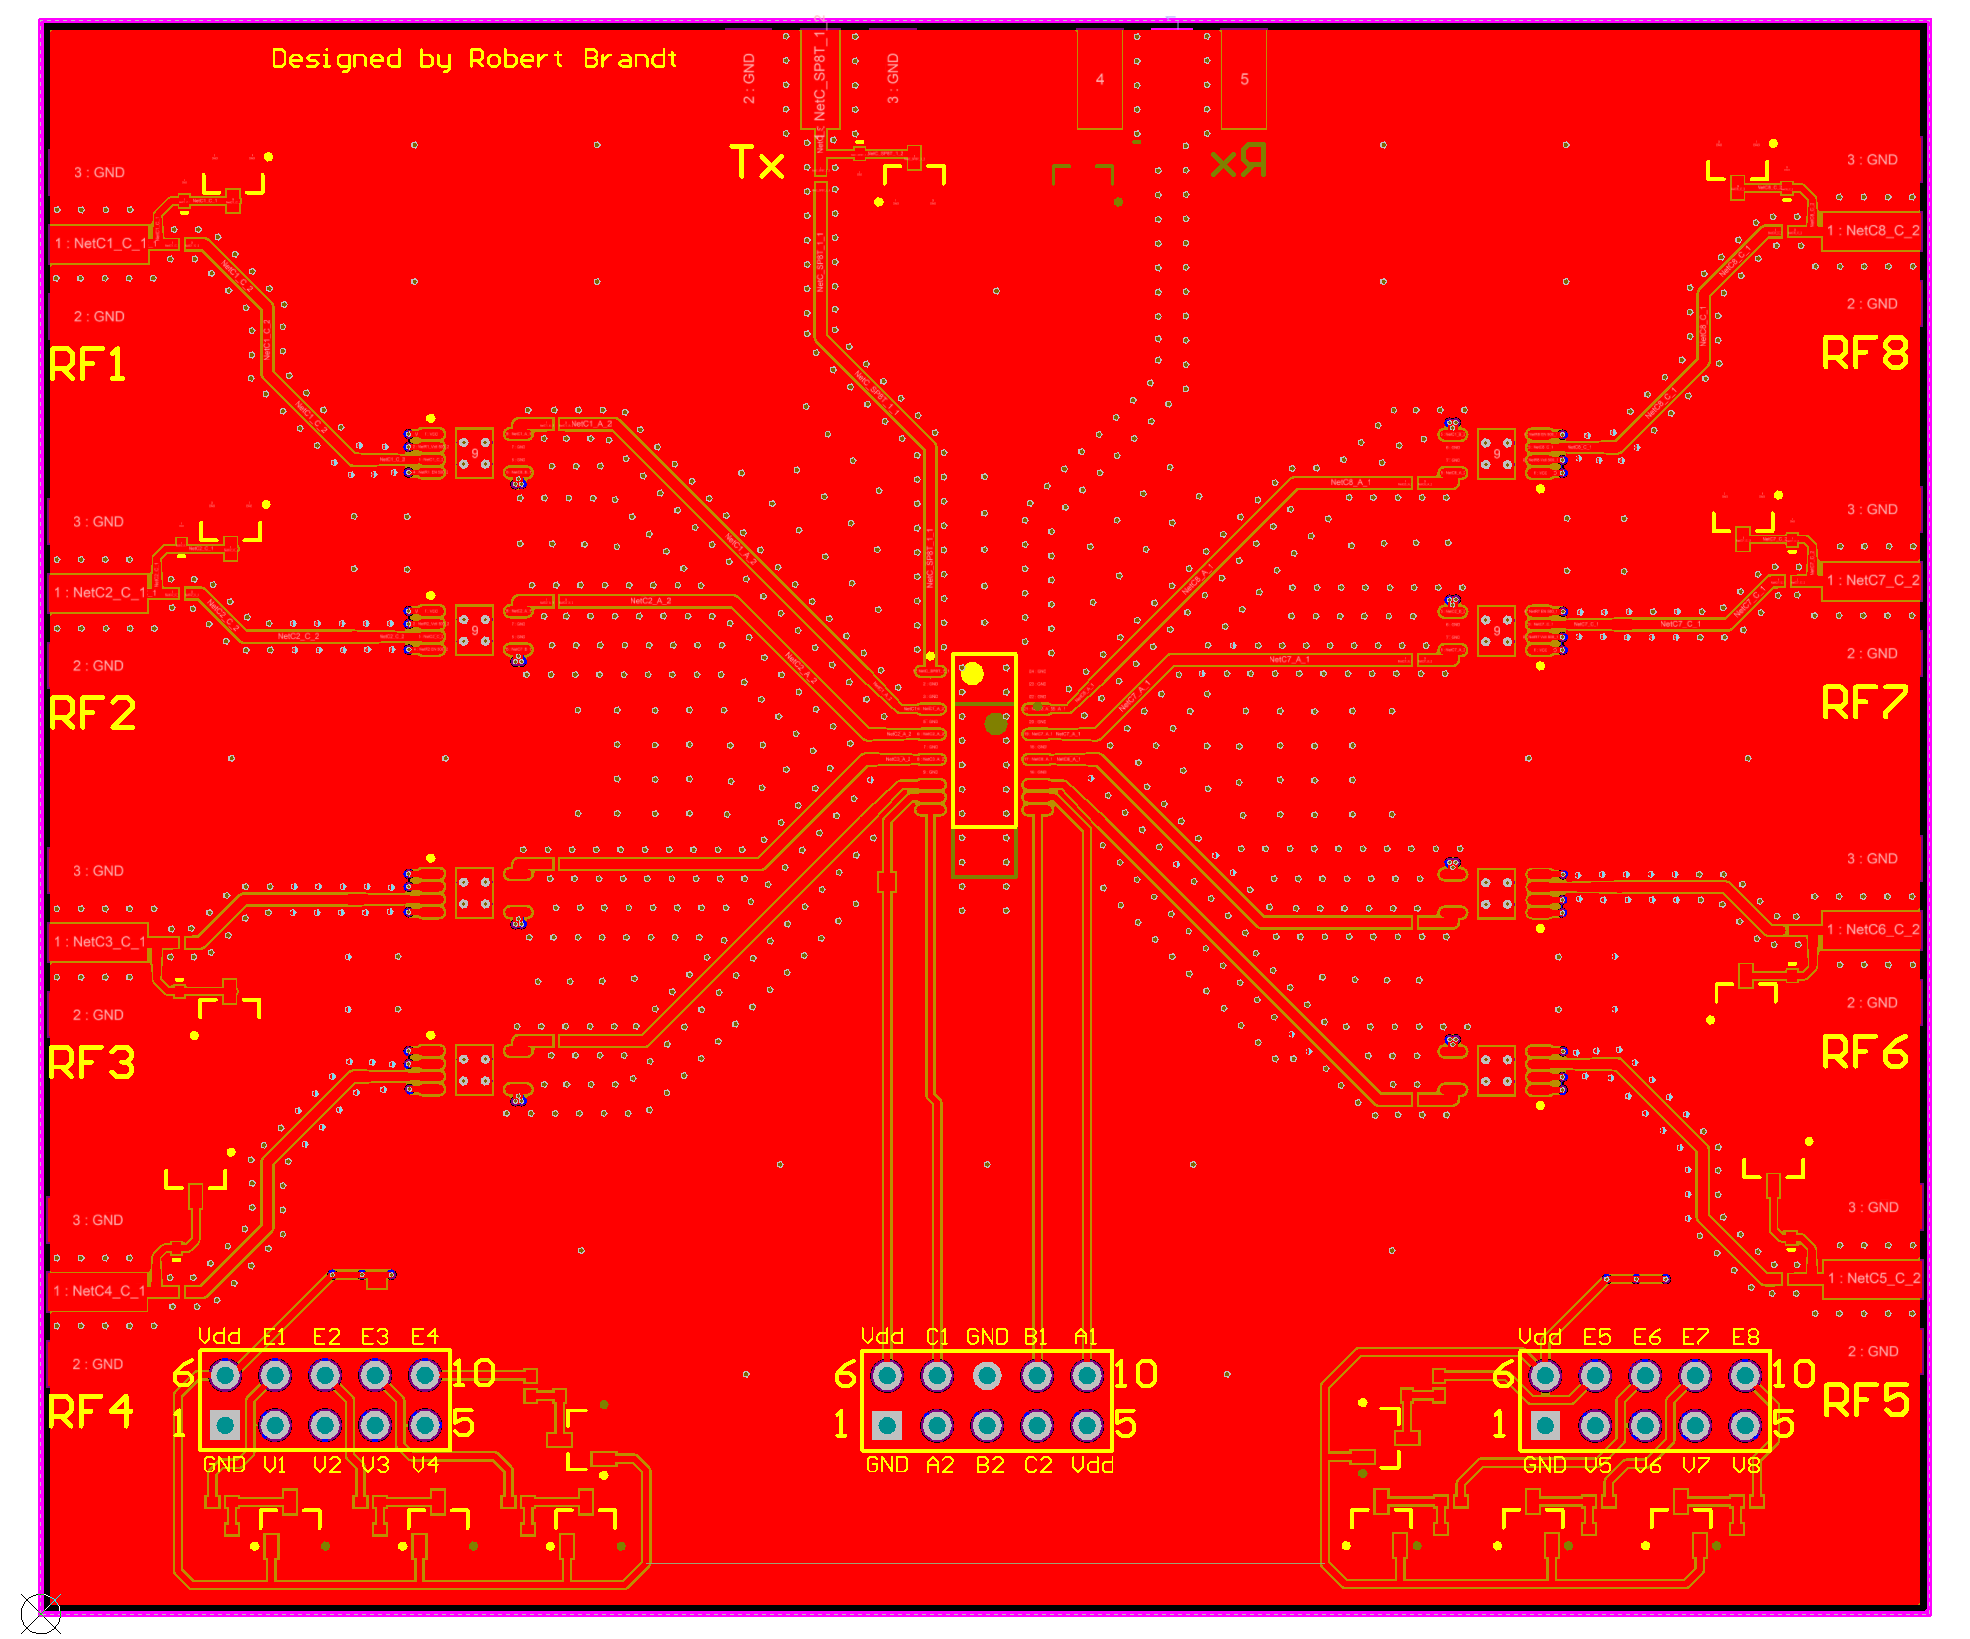
\includegraphics[width=5.5in]{./images/sp8t_top.png}
		\caption{PCB layout for top layer of SP8T and SPDT board}
		\label{fig:sp8t_top}
	\end{center}
\end{figure}

\begin{figure}[h]
	\begin{center}
		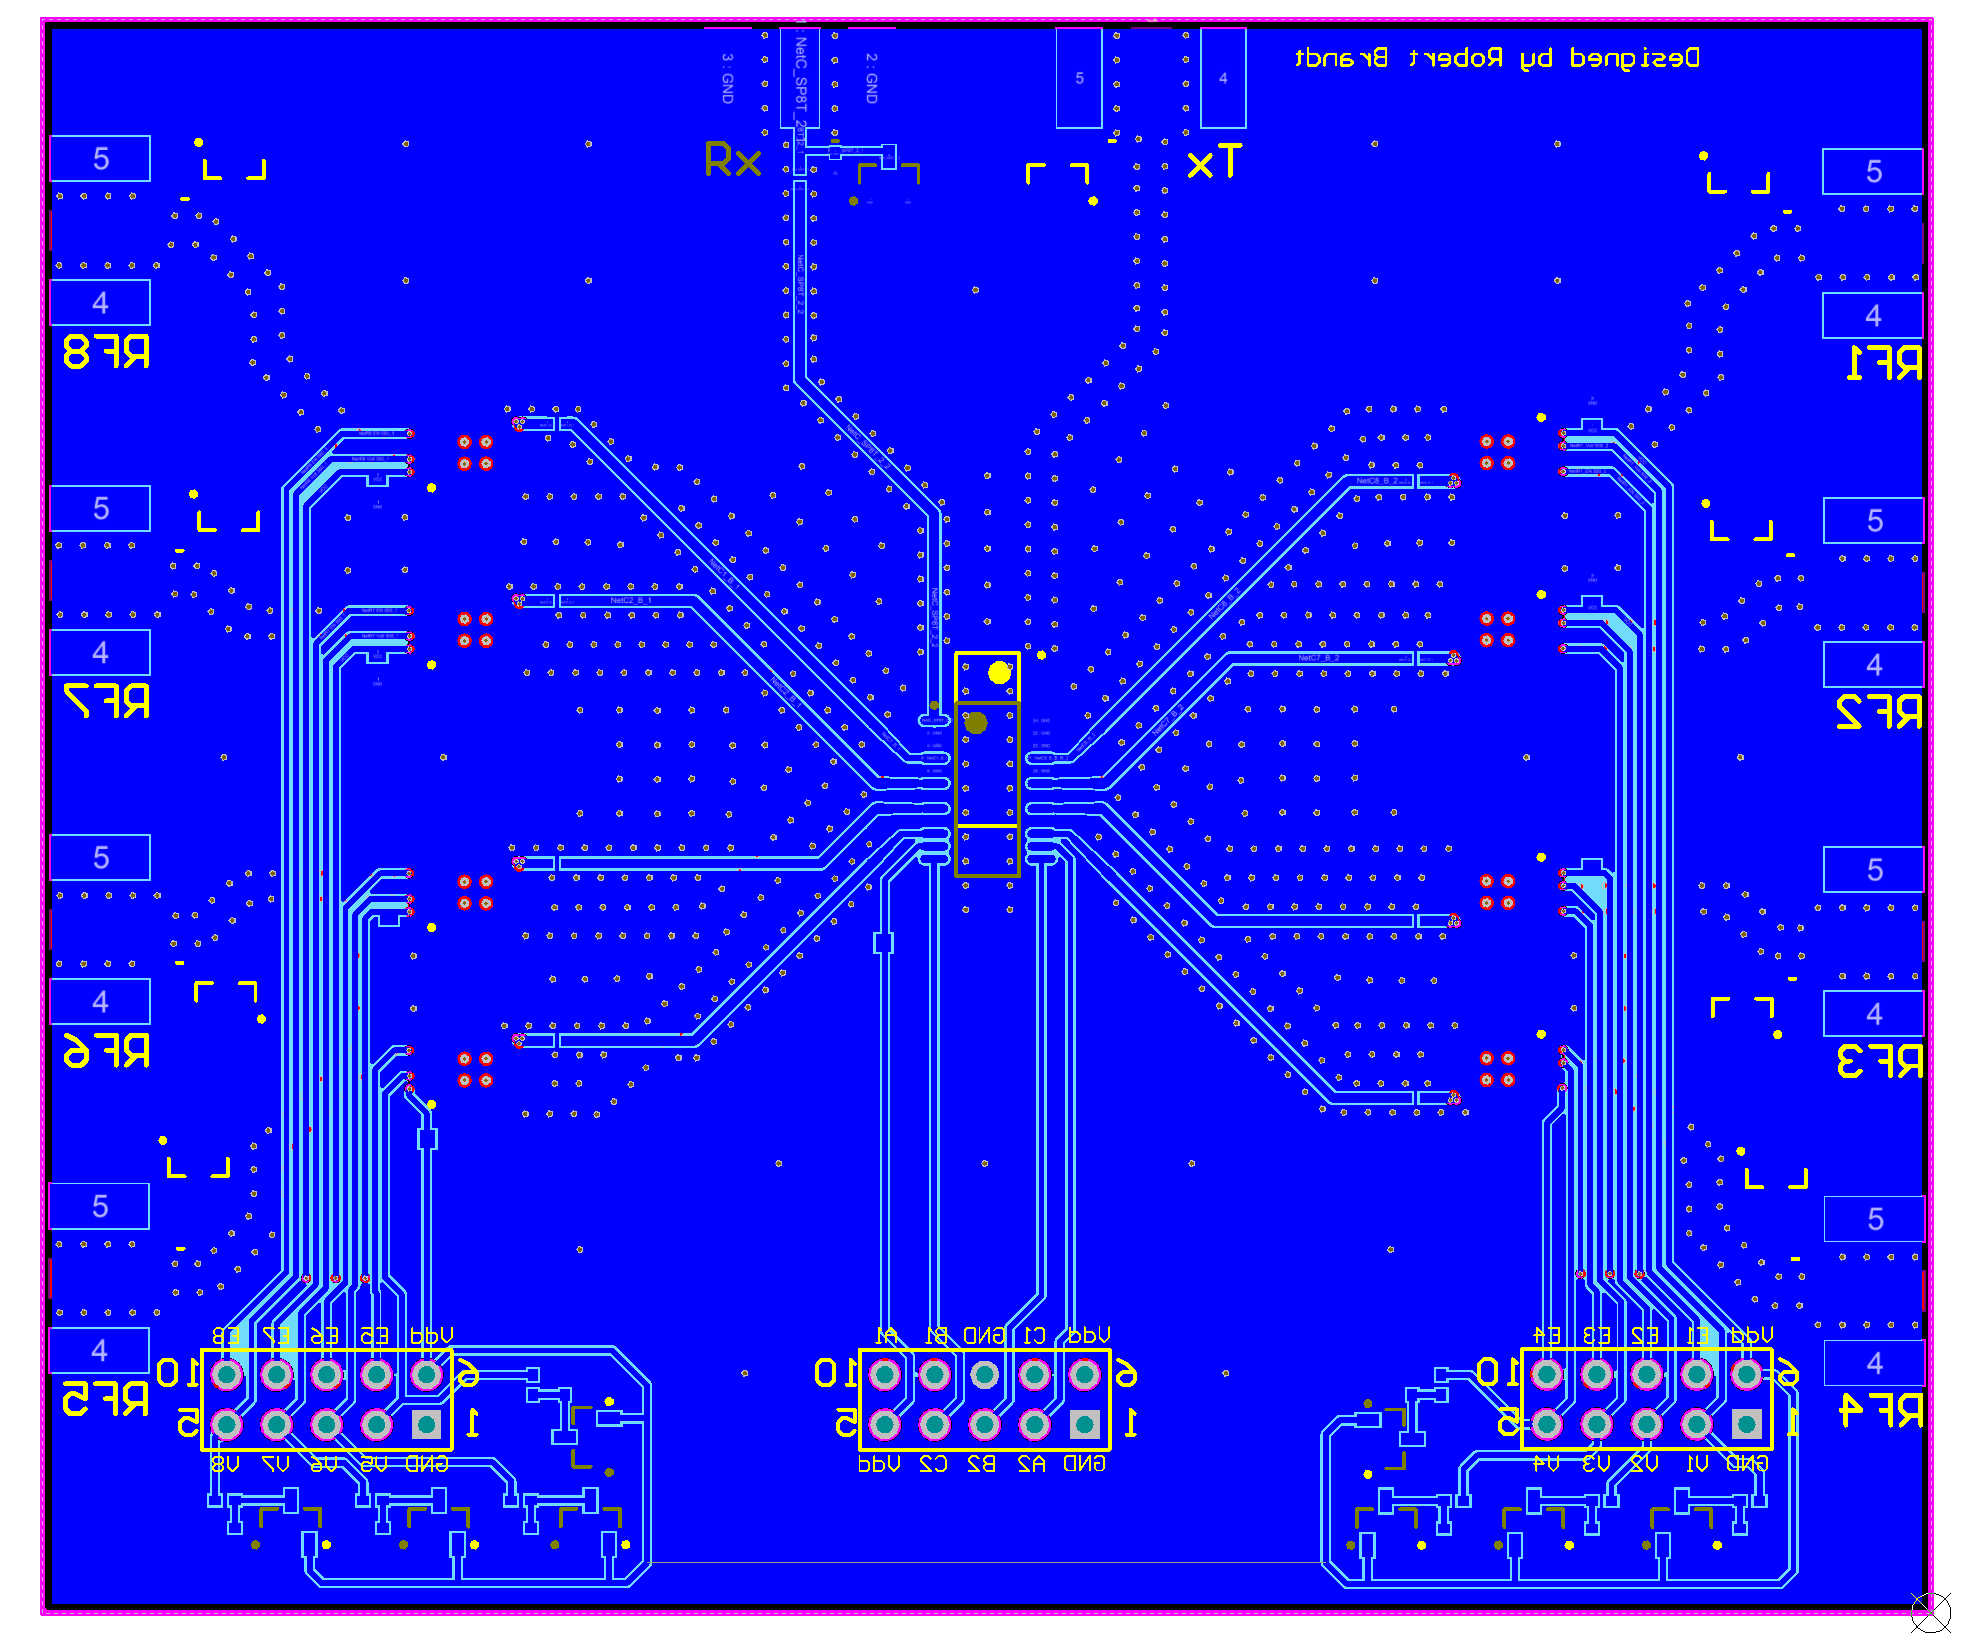
\includegraphics[width=5.5in]{./images/sp8t_bottom.png}
		\caption{PCB layout for bottom layer of SP8T and SPDT board}
		\label{fig:sp8t_bottom}
	\end{center}
\end{figure}

\begin{figure}[h]
	\begin{center}
		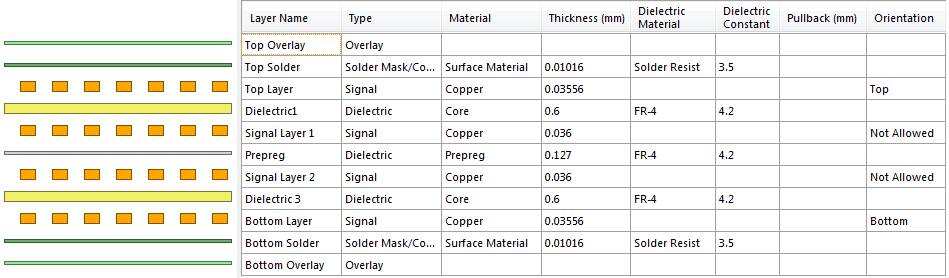
\includegraphics[width=5in]{./images/stackup.png}
		\caption{Stack up for PCBs in Altium}
		\label{fig:stackup}
	\end{center}
\end{figure}


Unfortunately, due to issues with our original intended supplier of our PCBs, we were unable to get these PCBs printed in time for this report. We found another supplier for our PCBs and hope to have them before our presentation. The PCBs needed to be modified somewhat due to different PCB specifications from this new supplier. Minimum routing size was larger at 0.1524 mm compared to 0.1 mm with the original supplier. Also, the substrate thickness options were different, not allowing us to use a thickness of 0.6 mm. Based on the specifications of the new supplier the RF traces needed to be modified to 0.185 mm thick with a gap of 0.1524 mm. This is based on a substrate thickness of 0.1 mm.


	%!TEX root =  ../final-report.tex

% Chapters are setup to start on a new page.
% The short version of that title appears in square brackets. This is used for the table of contents listing. 
% The long version of the title has a command "\setstretch{0.5}" in order to reduce the line spacing in the
% title and then the title text.
\section{DC Switching and Power Integration}

DC circuits are commonly used for controlling RF switches due to the cheaper cost in comparison to their RF counterparts and the reduction in frequency interference due to the maximum attenuation of any frequency components at DC. For our design we need a DC circuit for address decoding of the RF switch. In effect, the function of the DC switch is to set the control parameters in order to specify what the response of the RF switch will be at that point in time. 

\subsection{Research and Design}

\subsubsection{DC Switch}

At the onset of the project, we examined the previous switch design to understand how it would integrate with the RF switch and set the control parameters for the acquisition of data by the VNA. Our goal was to improve upon this design so that it was feasible with the new system we wanted to implement.

\subsubsection{Hardware}

The initial design appeared very complex and cumbersome to deduce because it had wires everywhere. The first task was therefore to ascertain the possibility of having a neater hardware with very minimal adjustment to the circuit after the printing of the PCB. This meant that most of the design should be implemented in the PCB in order to reduce complexity and make troubleshooting easier. This also ensure a reduction in noise cause by all the numerous wiring and addition electrical components that was everywhere.

Figure \ref{fig:eddie_fig1} highlights that function of the DC switch in perfect simplicity. The control parameters are letters from A – L and these are sourced from the DC switch to the SP3Ts, SP3Ts and SPDTs of the RF switch

\begin{figure}[h]
	\begin{center}
		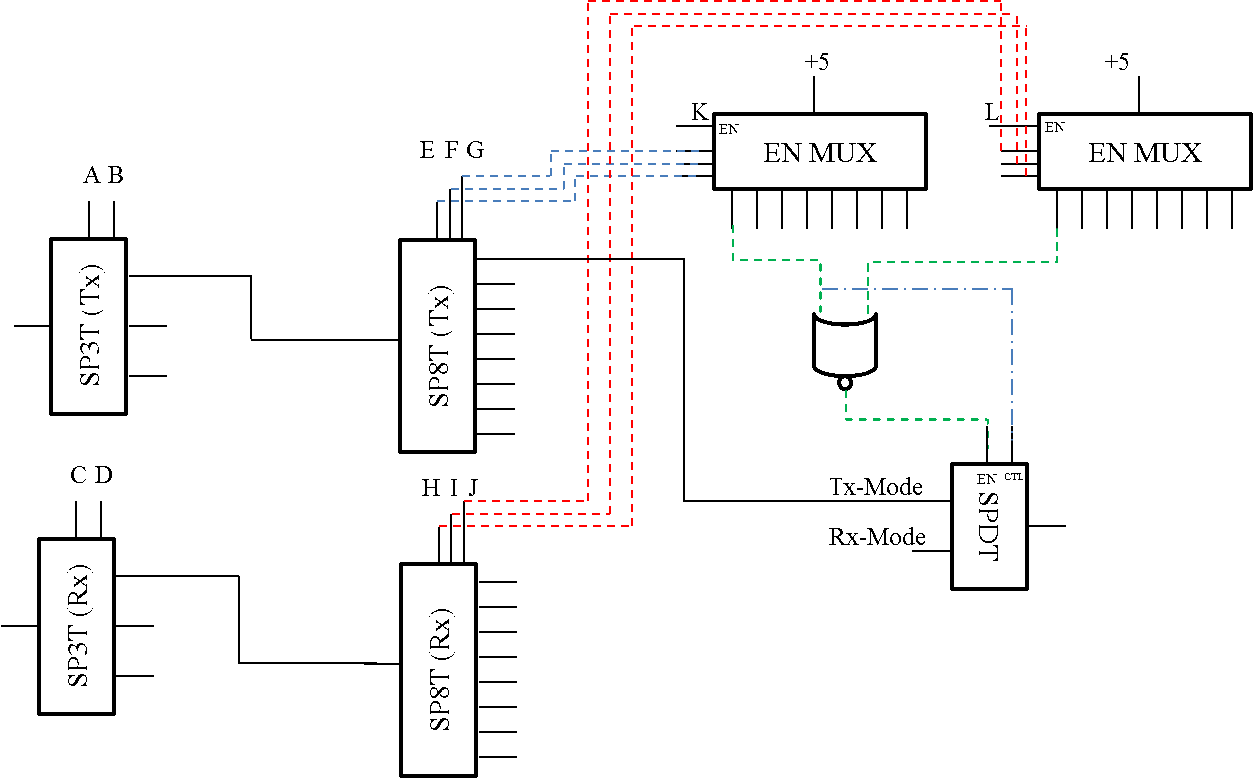
\includegraphics[width=4.5in]{./images/eddie_image1.png}
		\caption{}
		\label{fig:eddie_fig1}
	\end{center}
\end{figure}


\subsubsection{Software}

The software control of the DC switching circuit is done by an Arduino microcontroller loaded with a table that references the control lines for each multiplexer. This allows the SPDTs to function as an input or an output depending on the values set on the control lines but the Arduino. And will be concurrent with the presents action of the VNA such that, only one SPDT is in transmit mode at a given time. The software will also turn on one the SP8T for transmission of the signal and turn the other SP8Ts responsible for reception of the signals. 

After the research and understanding of requirements were satisfied, a truth table was drawn in order to simplify the circuit to its least possible scenario where the fewest components are used to achieve the expected results. This truth table was then transcribed into code for and then loaded unto the Arduino. This Arduino was set to function in synchronism with the raspberry pie.

\subsubsection{ESD Protection}

Any reliable system design requires some form of Electrostatic Discharge protection. Choosing the right circuit protection device involves considering criteria such as: Response time, ESD current handling capacity and, maximum reverse leakage current. Also the device should not interfere with the normal operation of the circuit. Designing the DC circuit also meant taking the RF circuit into consideration in order to minimize electrostatic discharge and current leakage. 

We considered N-well resisters, gate-grounded and gate-coupled protection options, silicon controlled rectifiers and diodes. Ultimately we decided to use diodes and capacitors due to its simplicity.

\subsubsection{Power Integration}

A portable power source will be integrated into our data collection unit to provide enough electrical power to run the VNA and the switch box simultaneously for the duration of time it takes to gather the parametric information from the VNA. 12V rechargeable battery which produces 3.0Ah of current will be hour choice as our power source.

\subsection{Design and Implementation}

\subsubsection{DC Switch}

The design of the switch required the use of Altium and the Arduino user interface. The hardware was designed in Altium and the software was writing in the Arduino mainframe in the C++ programing language 

\subsubsection{Hardware}

Designing the PCB first started with the schematic and a review of the schematic to ensure its accuracy. Figre \ref{fig_eddie_fig2} shows the final schematic that was used in the printing of the PCB in Altium.

\begin{figure}[h]
	\begin{center}
		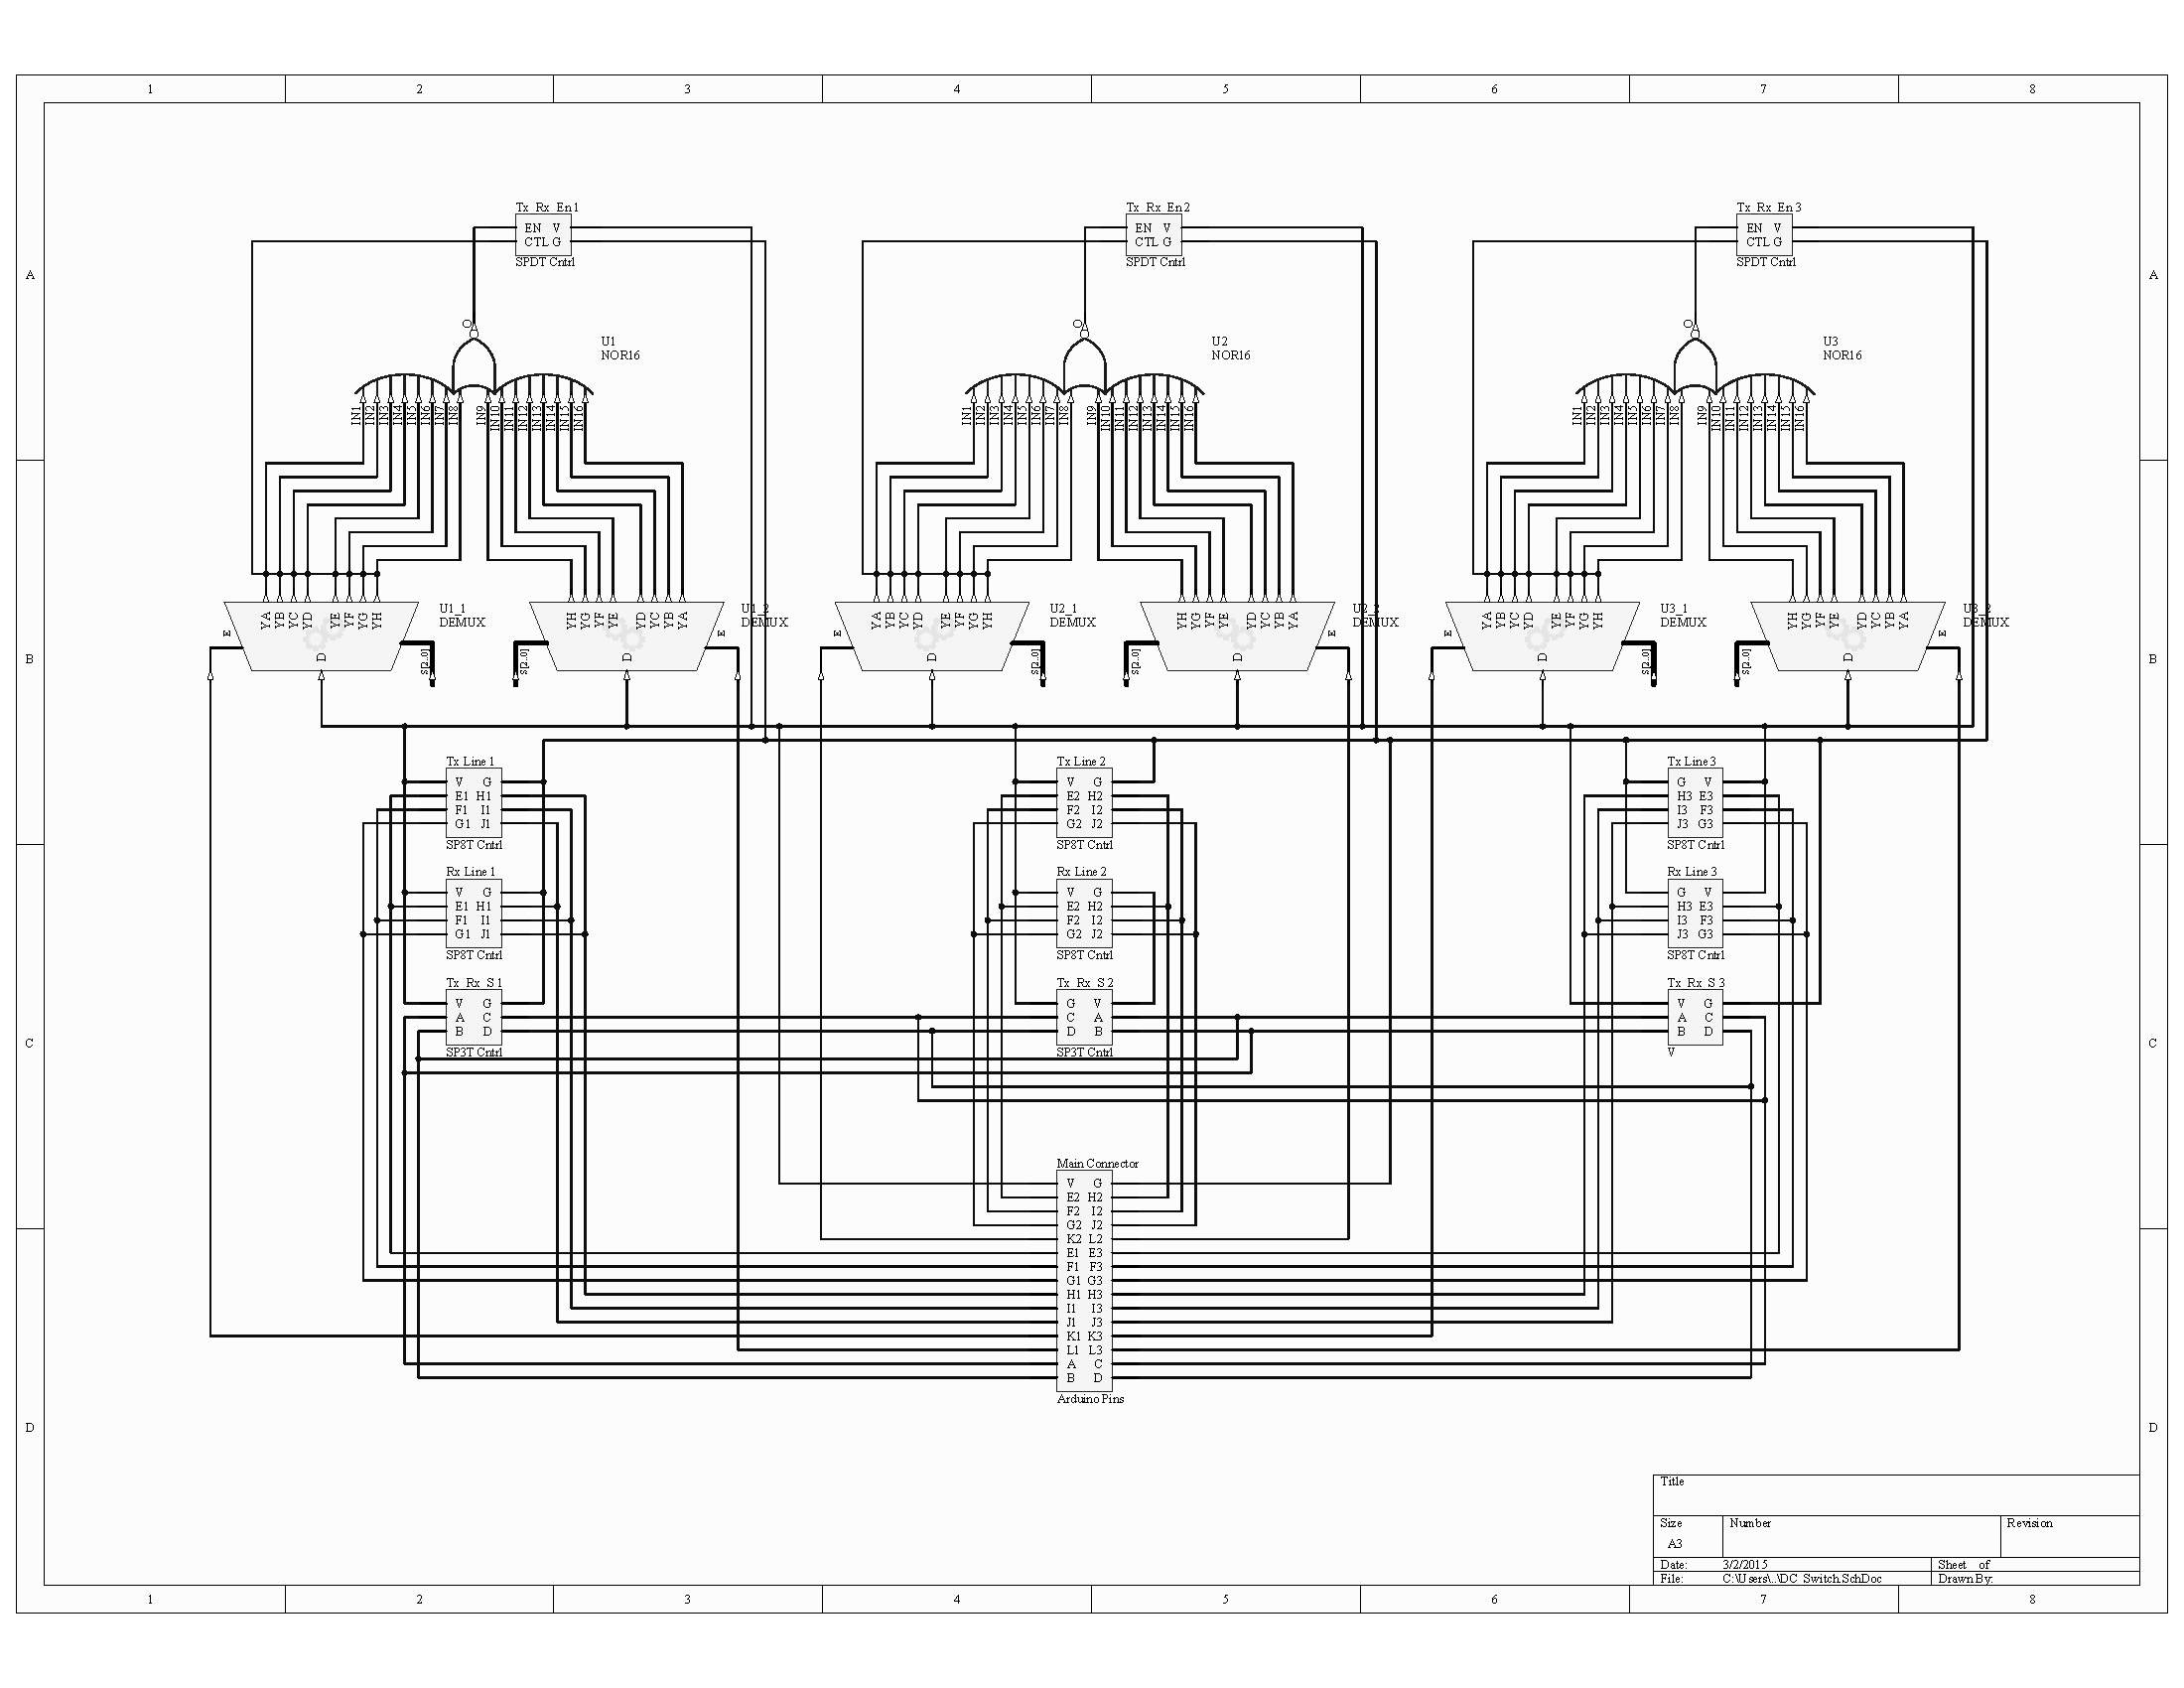
\includegraphics[width=5.5in]{./images/eddie_image2.png}
		\caption{}
		\label{fig:eddie_fig2}
	\end{center}
\end{figure}










	%!TEX root =  ../final-report.tex
%
% Chapters are setup to start on a new page. The short version of that title appears in square brackets. This is used for the
% table of contents listing. The long version of the title has a command "\setstretch{0.5}" in order to reduce the line
% spacing in the title and then the title text.
\chapter{Vector Network Analyzer}
\label{sec:VNA}

The vector network analyzer is a key component of the S-Parameter Data Acquisition (SPDAQ) system since it is the actual
instrument that measures the S-Parameters of the grain storage unit.

% Sections will automatically be numbered by LaTeX.
\section{Harware Specifications}

In order to implement a practical system that would be ideally used by agriculturalists such as farmers, the VNA had to be
portable yet affordable. Lab quality VNAs are very expensive, usually costing tens of thousands of dollars, and therefore
cannot be used for the SPDAQ system. Due to the fairly low frequencies being transmitted and received from the antennas
within the grain storage unit, the VNA can be more affordable than those usually found in a lab.  On top of these main
specifications of a compact, low-costing VNA, the analyzer had to be a two port system so it is capable of S11 and S12
measurements for the microwave imaging of the grain bin,as well as being capable of measuring within the frequency range of a typical grain bin,and can offer a good dynamic range.  Table \ref{table:vna} shows the exact specifications required for the SPDAQ system to be effective.
\clearpage{}
\begin{table}[!h]
\centering
\caption{VNA Requirements \cite{vnaspecs}}
\label{table:vna}
\begin{tabular}{|l|l|}
\hline
Frequency Range & 70 MHz - 100 MHz 			\\ \hline
Dynamic Range   & ≥ 10 dB          			\\ \hline
System Type     & 2-port with S11 and S12 	\\ \hline
Budget   		& \textless \$1000		\\ \hline
\end{tabular}
\end{table}

These criteria help facilitate in the decision of selecting the MiniVNA Pro (MVP) by Mini Radio Solutions which offers a more affordable and portable solution for the VNA component of the SPDAQ system.

\begin{table}[!h]
\centering
\caption{miniVNA PRO Specifications}
\label{table:mvp}
\begin{tabular}{|l|l|}
\hline
Frequency Range & 0.1 MHz - 200 MHz                                                                             \\ \hline
Dynamic Range   & \begin{tabular}[c]{@{}l@{}}90 dB in Transmission mode\\ 50 dB in Reflection mode\end{tabular} \\ \hline
System Type     & 2-port with S11 and S12                                                                       \\ \hline
Cost            & \$549.95 + taxes and fees							\\ \hline
\end{tabular}
\end{table}

As shown in Table \ref{table:mvp}, the MVP meets all the main VNA requirements for the SPDAQ system which made it a valid solution
for the VNA component.
\clearpage{}
\section{Calibration and Testing}

To ensure that the MVP meets our system’s standards, results measured from the MVP were compared to the more high-tech VNAs
in the Electromagnetic Imaging Lab (EIL) that are normally used for the imaging data.  The MVP is first calibrated using the calibration tool provided by the EIL and calibration files are created using the MVP software, which is shown in Figure \ref{fig:calib}.
\newline
\begin{figure}[!ht]
\begin{center}
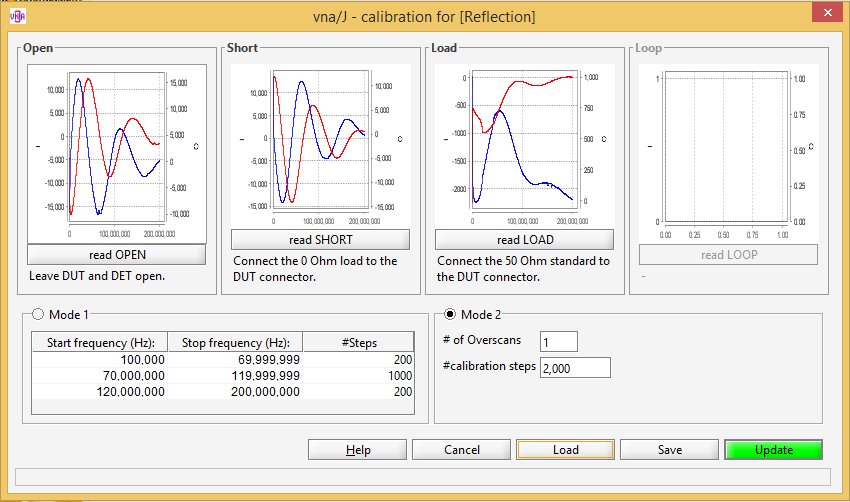
\includegraphics[width=4.9in]{./images/calib.png}
\caption{miniVNA PRO calibration software.}
\label{fig:calib}
\end{center}
\end{figure}

The S11 measurement of the miniVNA PRO was then compared to the S11 measurement of the EIL VNA in order to verify the calibration was performed correctly on the miniVNA PRO. The RF Switch module provided by the EIL was used as a load. The S11 output of the RF Switch transfer function is shown in Figure \ref{fig:real} and \ref{fig:imag} for both the EIL VNA and the miniVNA PRO. Both the real and imaginary part of the S11 measurement are fairly similar with a slight discrepancy in the real part of S11 in the miniVNA PRO which may be due to the calibration kit used with the miniVNA Pro since the kit was designed for the EIL VNAs. 
With fairly accurate results, the MVP gave us confidence in using it for the SPDAQ system. 

\begin{figure}[!ht]
\begin{center}
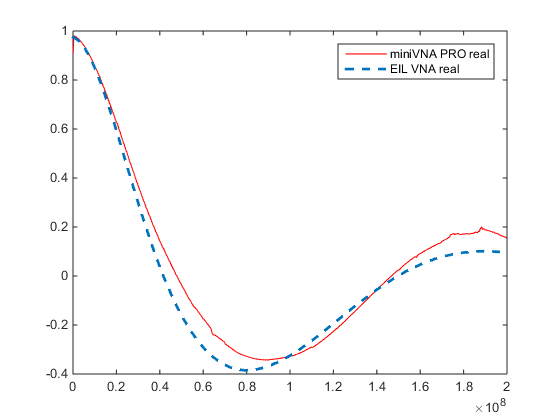
\includegraphics[width=3.8in]{./images/real.png}
\caption{S11 measurement(real) for both VNAS.}
\label{fig:real}
\end{center}
\end{figure}

\begin{figure}[!ht]
\begin{center}
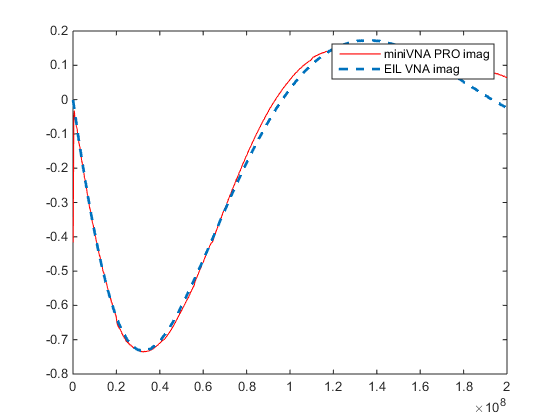
\includegraphics[width=3.8in]{./images/imag.png}
\caption{miniVNA PRO open port measurement in reflection mode.}
\label{fig:imag}
\end{center}
\end{figure}

\clearpage{}
\section{miniVNA PRO Software}

The MVP was designed to be software-defined and the manufacturer did not have any indications that they will make this device
open source. This forced our team to go ahead with the manufacturer’s software in order to use the MVP despite the slow read
times of each measurement.
\newline

\begin{figure}[h]
\begin{center}
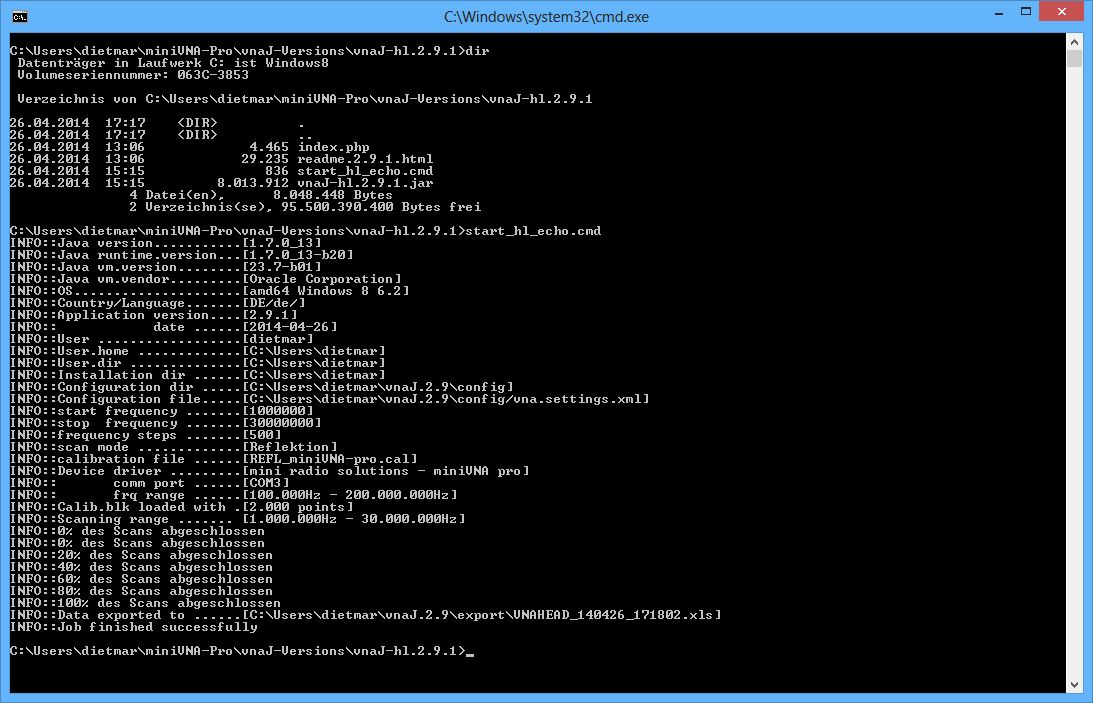
\includegraphics[width=4.5in]{./images/cli.jpg}
\caption{miniVNA PRO Software Output}
\label{fig:cli}
\end{center}
\end{figure}

The MVP’s software used for the SPDAQ system is the ‘vnaJ-hl.3.1.3.jar’ file [3] that runs on a headless system (no graphical
user interface). When the jar file is executed with the specified parameters (frequency start, stop and steps), the MVP takes
the readings and exports them to a CSV file (the file type is specified within the parameters of the jar file).  An example
output of the MVP’s software running through a command line interface (CLI) is shown in Figure \ref{fig:cli}.



\chapter{Microprocessor}
\label{sec:software}

% Sections will automatically be numbered by LaTeX.

\section{Hardware Integration}

Due to the software limitation of the MiniVNA Pro (MVP), a microprocessor was required to run the MVP’s software. This is
where the Raspberry Pi 2 (RPi 2) was chosen.  The RPi 2 microprocessor will be used to control both the RF Multiplexer and
MiniVNA Pro (MVP) of the S-Parameter Data Acquisition (SPDAQ) system.  The specifications of the RPi 2 are shown in Table
\ref{table:RPi2}.

\begin{table}[h]
\centering
\caption{Raspberry Pi 2 Specifications \cite{RPi2}}
\label{table:RPi2}
\begin{tabular}{|l|l|}
\hline
Processor & 900Mhz quad-core ARM Cortex-A7 CPU 	\\ \hline
RAM       & 1GB									\\ \hline
USB Ports & 4                                  	\\ \hline
GPIO Pins & 40				\\ \hline
\end{tabular}
\end{table}

The RPi2 offers enough USB ports to connect the RF Multiplexer (RF Mux) and MVP.  As well, the RPi2 offers GPIO pins, which will be used to integrate user interface (UI) features for the user to have better control of the system.  Such UI features that were
implemented with the RPi2 was a button to run the SPDAQ’s software when pressed and a LED indicator to allow the user to know
when the program is ready for the user to press the button.  A circuit is shown in Figure \ref{fig:button} that displays the button
and LED connection to the appropriate GPIO pins on the RPi2 (see Appendix \ref{appendix:rpi2} for Raspberry Pi 2 Pinout Configuration).

\begin{figure}[h]
\begin{center}
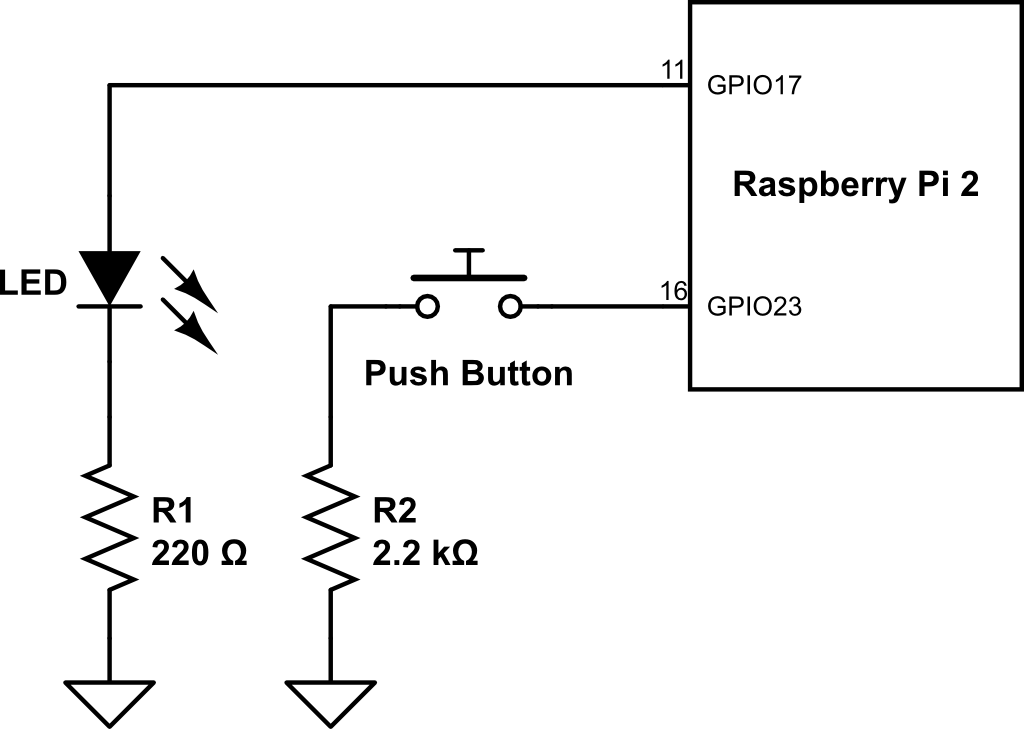
\includegraphics[width=3.8in]{./images/rpi2.png}
\caption{LED and Button Circuit}
\label{fig:button}
\end{center}
\end{figure}

Initially, the SPDAQ system was designed around the Raspberry Pi Model B+ but due to the new release of the RPi 2 in
February, 2015, the decision to upgrade seem obvious with the faster processor at the same low cost of 39.99 CAD + shipping
that the old Raspberry Pi Model B+ was priced at.  The hardware upgrade helped greatly improve the software run times down to
16s per measurement to ~5s per measurement.  Boot up times for the system also greatly reduced to 6s from 15s.

\section{Software Design and Integration}

Arch Linux was installed onto the RPi 2 due to its minimal architecture. It is a lightweight operating system (OS) that is
text-based with no GUI making it very quick to boot up.  Since the SPDAQ system has no need for a GUI and the software that
will be running on the RPi 2 did not require much to run, the Arch Linux OS provided a great solution for our system.

For the SPDAQ system, there are four main processes that the system is required to run: Initialization, Data Acquisition,
Post-Data Processing, and Remote Data Accessing. The order of all these processes and procedures that run on the
microprocessor are shown in Figure \ref{fig:procs}.

\begin{figure}[h]
\begin{center}

\includegraphics[width=5.4in]{./images/procs.png}
\caption{S-Parameter Data Acquisition system processes.}
\label{fig:procs}
\end{center}
\end{figure}

\subsection{Initialization Process}

The initialization process requires the user to interact with the system to power on and start the other processes that are
executed by a shell script.  The procedure is as follows:

\begin{enumerate}
\item Power on the S-Parameter Data Acquisition (SPDAQ) system by connecting the RPi2 to a power source.
\item Once booted up (allow approximately 7s), the user can now press the push button to execute a shell script that will start the data acquisition process.
\end{enumerate}

\subsection{Data Acquisition Process}

In this process, the RPi 2 will control both the RF Multiplexer to switch the antennas between transmitter and receiver as
well triggering the MVP to execute a sweep to obtain S-Parameters of the Grain Bin.  The Data Acquisition Process runs
through an N-number antenna array collecting the S-parameter data from the grain bin through the use of the MVP, which
exports a CSV file per sweep.  Each antenna will act as a transmitter and will loop through all n number of antennas acting
as a receiver, which results in an N x N number of measurements.  This will also result in N x N number of exported data
files from the MVP due to its software limitations.  These data files are exported to
/root/vnaJ.3.1.3/export directory of the RPi2.  A flow chart of the Data
Acquisition Process is shown in Figure \ref{fig:switch} which outlines this procedure.

\begin{figure}[h]
\begin{center}
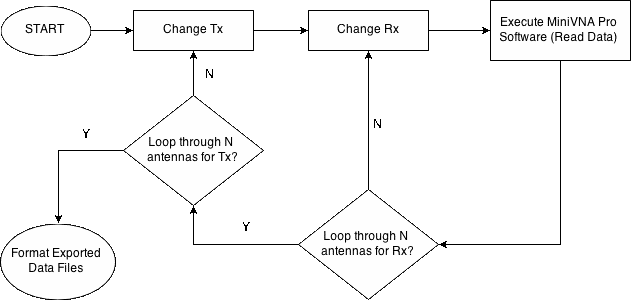
\includegraphics[width=5in]{./images/switch.png}
\caption{Flow chart of the Data Acquisition Process.}
\label{fig:switch}
\end{center}
\end{figure}

\subsection{Post-Data Processing}

Post-Data Processing procedure is executed by the shell script after the Data Acquisition Process is done.  In this process,
the exported CSV files from the MVP are reformatted to a single data file, which the user can access for further processing
such as microwave imaging analysis of the grain bin.  The exported CSV files are located in the
/root/vnaJ.3.1/export directory with the filename format of
$gbin_{tx}{rx}.csv$ where “{tx}” and “{rx}” are the 2-digit transmitter and receiver antenna number, respectively, within the
array that the MVP measured from. The MVP exports the data as transmission loss in dB and transmission phase (degrees), which
is S12 in polar form, however Cartesian complex form is required for post-analysis and therefore a small calculation is
required prior to writing to file. The calculations performed are described below:
\clearpage{}
\noindent
The MVP provides its data as so, 
\\$Transmission Loss (TL)=20\log_{10}|S12| Transmission Phase= \theta$
\noindent
The desired data form is as so, $S12=a+bi$
\noindent
Variables a and b are calculated as shown, 
\\$a=|S12|\cos\theta b=|S12|\sin\theta where,|S12|= 10^{(TL/20)}$

Once the S12 data is calculated to Cartesian complex format, it is then written to a file called “sp.dat” which is located in
/root/grainbin/output/ directory.  The format of the file is shown as:

\begin{verbatim}
Tx	Rx	Probe	    S12 Real	S12 Imaginary (repeating for all frequency steps)
\end{verbatim}

Where Tx is the transmitter antenna number and Rx is the receiver antenna number, which is then followed by the S12 real and
imaginary data in succession for all 100 frequency steps.  A flow chart of the Post-Data Processing procedure is shown in Figure
\ref{fig:pdp}.


\begin{figure}[h]
\begin{center}
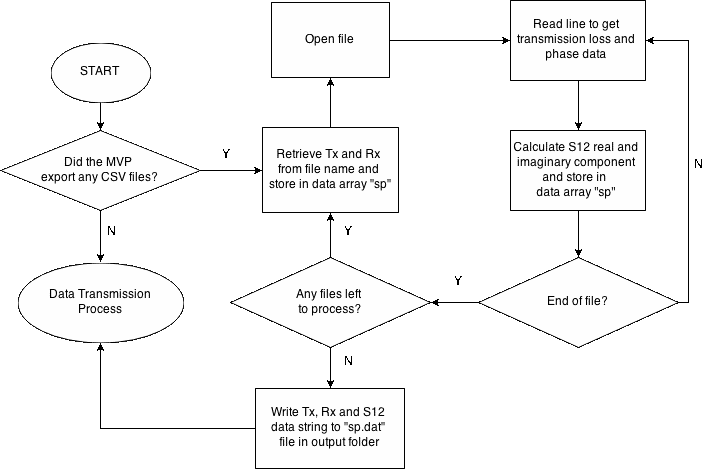
\includegraphics[width=5in]{./images/pdp.png}
\caption{Flow Chart of Post-Data Processing
Procedure.}
\label{fig:pdp}
\end{center}
\end{figure}

\subsection{Data Transmission Process}

The “sp.dat” file contains all of the S-parameters of the grain storage unit and this file will be accessible to the user
through the cloud if an Internet connection is present.  The shell script will execute the data upload process after the
Post-Data Processing is complete in which it executes a command in Linux that triggers an upload of the specific file to
Dropbox.

Dropbox is a widely used cloud storage service that anyone can register for free for basic cloud storage space. This service
can be accessed online remotely from the users own PC through the many interfaces that Dropbox offers (ex. website, computer
software, etc.), which makes it very convenient for the user to retrieve the data from the SDAS and therefore was selected
for our system.  Appendix \ref{appendix:dropbox} instructs how a user can unlink or link a specific Dropbox account onto the RPi2 as well as
additional commands.

However, if the SPDAQ system is unable to connect to the Internet to upload the data file, the user can still manually
retrieve the data through the following methods:

\begin{enumerate}
\item Ejecting the micro-SD card located underneath the RPi2 in which the file is stored on.
\item SFTP with the RPi2 through an Ethernet connection with another device.
\begin{itemize}
\item The RPi2 is assigned a static IP address for the user to SSH and SFTP in order to communicate with it. That static IP address is: \textit{192.168.2.23}.  Once SFTP establishes a connection, executing the command, \textit{“get /root/grainbin/output/sp.dat”} will transfer the file over to the users remote device.
\end{itemize}
\end{enumerate}

\section{Software Setup and Configuration}

This chapter section details the software setup and configuration on the RPi2 to run the SPDAQ software. The purpose of this
section is to help a user recreate the SPDAQ software on the RPi2 in the case of any software error or corruption or to
simply modify specific software parameters to tailor to the user’s needs.

\subsection{Prerequisites} The RPi2 is setup with a username and password.  The default login information for Arch Linux is
the following:

\begin{verbatim}
Username: root 
Password: root
\end{verbatim}

However for security purposes, the password was changed to 'gbin2015' with the same username.
\newline
In order for the RPi2 software processes to function, certain files need to be included on the RPi2 stored in the directory
/root/grainbin. A list of these files is shown in Table \ref{table:files}

\begin{table}[h]
\centering
\caption{Required files in the /root/grainbin directory of the Raspberry Pi 2.}
\label{table:files}
\resizebox{\textwidth}{!}{%
\begin{tabular}{|l|l|}
\hline
\textbf{File}		& \textbf{Description} 																						\\ \hline
vnaJ-hl.3.1.3.jar   & miniVNA PRO headless software 																			\\ \hline
gbin.sh 			& shell script t run all of the SPDAQ processes (see Appendix \ref{appendix:gbinsh}) 								\\ \hline
dropbox-uploader.sh & Dropbox shell script to upload "sp.dat" file to a linked Dropbox account on the RPi2 (see Appendix \ref{appendix:dropbox})   																										\\ \hline
put2str.exe         & processes the exported CSV files from the miniVNA PRO (see Appendix \ref{appendix:put2str}) 						\\ \hline
button.py 			& button and LED function on the Raspberry Pi 2 (see Appendix \ref{appendix:button})	\\ \hline
\end{tabular}
}
\end{table}

Specific packages also need to be installed onto the RPi2 for the files to run properly on the Arch Linux OS. The following
commands shown in Table \ref{table:pkg} can be executed on the RPi2 terminal with Arch Linux installed.  Ensure that the RPi2 is connected to the Internet in order to download these packages.

\begin{table}[h]
\centering
\caption{Required packages to be installed on Arch Linux OS running on the Raspberry Pi 2.}
\label{table:pkg}
\begin{tabular}{|l|l|}
\hline
\textbf{Command}				& \textbf{Description} 				\\ \hline
pacman –S jdk7-openjdk			& Java package 						\\ \hline
pacman –S mono                  & C\# Compiler                     	\\ \hline
pacman –S python-raspberry-gpio & Raspberry Pi GPIO Python library	\\ \hline
\end{tabular}
\end{table}

Once the packages are installed, the MVP’s software requires specific directories to be created. These directories are
created when the ‘vnaJ-hl.3.1.3.jar’ file is executed for the first time which can be executed using the following command:

\noindent
\textbf{\textit{ java –Dconfigfile=gbin.xml -Dfstart=70000000 -Dfstop=100000000 -Dfsteps=100 -Dcalfile=gbin.cal -Dscanmode=TRAN -Dexports=csv -jar vnaJ-hl.3.1.3.jar}}

An error will occur due to certain files missing when the command is executed for the first time however the necessary
directories will be created on the /root directory of the RPi2 which includes:
\setlist{noitemsep}
\begin{itemize}
\item /root/vnaJ.3.1/export
\item /root/vnaJ.3.1/calibration
\item /root/vnaJ.3.1/config
\end{itemize}

There are two key files that need to be present for the ‘vnaJ-hl.3.1.3.jar’ file to execute properly.  The first one is the
configuration file “gbin.xml” which can be found in Appendix \ref{appendix:xml}.  The XML file includes the USB port name for the software to
communicate with the MVP. This file must be stored in the /root/vnaJ.3.1/config directory. The second key file is the
calibration file for transmission mode which are created using the ‘vnaJ.3.1.3.jar’ GUI software that must be run on a
separate computer that supports either Mac OS or Windows.  The user should consult the vnaJ software user manual \cite{vnaj} for
details on how these calibration files are created using the ‘vnaJ.3.1.3.jar’ GUI. This calibration file is stored in the
\noindent
\textit{/root/vnaJ.3.1/config} directory.
\newline
The RPi2 is now setup to run the ‘gbin.sh’ shell script that runs the SPDAQ software.   In order to use the button and LED
feature, the python script ‘button.py’ needs to be executed. The simple command “Python button.py” will run the python script
and will listen for the user to press a button to initiate the ‘gbin.sh’ script.  In order to setup the python script
‘button.py’ at bootup, the following command can be entered on the terminal of the RPi2:

\textbf{\textit{crontab –e}}

\noindent 
A file will come up and in this file enter in the line at the very bottom:

\textbf{\textit{@reboot python /root/grainbin/button.py}}

\noindent
Save the file and now the RPi2 will run the python script at bootup, enabling the button and LED function. To connect the LED and push button to the RPi2, review Figure \ref{fig:button} and Appendix \ref{appendix:rpi2} for GPIO pinout on the RPi2. 

\subsection{Configuration Parameters}

\subsubsection{‘gbin.sh’ Parameters}

The 'gbin.sh' shell script file is designed to take 4 parameters that define the number of transmitters and receivers being
used with the SPDAQ system.  The command to run the 'gbin.sh' file through the RPi2 terminal is:

\textbf{\textit{sh gbin.sh \{1\} \{2\}\ \{3\} \{4\}}}

\noindent
The 4 parameters are defined in Table \ref{table:gbinsh}.

\begin{table}[h]
\centering \caption{Parameter definitions for 'gbin.sh'.}
\label{table:gbinsh}
\begin{tabular}{|l|l|}
\hline
\textbf{Parameter} 	& \textbf{Description}             \\ \hline
\{1\}              	& transmitter antenna start number \\ \hline
\{2\}				& transmitter antenna stop number  \\ \hline
\{3\}     			& receiver antenna start number    \\ \hline
\{4\}              	& receiver antenna stop number			\\ \hline
\end{tabular}
\end{table}

An example of this command when using transmitter antennas 1-10 and antennas 11-20 as receiving,

\textbf{\textit{sh gbin.sh 01 10 11 20}}

\subsubsection{miniVNA PRO Software Parameters}

The MVP software is executed within the ‘gbin.sh’ shell script (refer to Appendix  \ref{appendix:gbinsh}) and the parameters can be changed by
changing the following command within that script:

\noindent
\textbf{\textit{java –Dconfigfile=gbin.xml -Dfstart=\{Start\} -Dfstop=\{Stop\} -Dfsteps=\{Steps\} 
\\-Dcalfile=gbin.cal -Dscanmode=TRAN -Dexports=csv -jar vnaJ-hl.3.1.3.jar}}

Where the following parameters are defined in Table \ref{table:vnaj}.

\begin{table}[h]
\centering
\caption{Parameter definitions for miniVNA PRO software command.}
\label{table:vnaj}
\begin{tabular}{|l|l|}
\hline
\textbf{Parameter} 	& \textbf{Description} 			\\ \hline
\{Start\}          	& Frequency range start (Hz) 	\\ \hline
\{Stop\}           	& Frequency range stop (Hz)		\\ \hline
\{Steps\} 			& Number of Frequency steps	\\ \hline
\end{tabular}
\end{table}

\noindent
The command is set within the shell script by default as:

\noindent
\textbf{\textit{java –Dconfigfile=gbin.xml -Dfstart=70000000 -Dfstop=100000000 -Dfsteps= 100
\\-Dcalfile=gbin.cal -Dscanmode=TRAN -Dexports=csv -jar vnaJ-hl.3.1.3.jar }}

\noindent
Where the frequency range is 70-100MHz with 100 steps.  The user can refer to the vnaJ Headless Software Manual
\cite{vnaJ-hl} for additional information.

\chapter{Future Work}

At the moment, the SPDAQ system is at an early stage of development. Our team has developed an Alpha prototype of the SPDAQ
system for hardware and software testing in order to establish a proof of concept for this project. Although our team was
successful in integrating the many hardware and software components for the system, there are still many things that can be improved on to make the system accessible to the general public. Initial designs for the SPDAQ system was to implement a battery operated device however due to project time constraints and project delays, this feature has yet to be implemented but should considered for future iterations. This chapter will explain the possible work that can be
done to advance the current alpha prototype of the SPDAQ system and its individual components.

\section{Software}

As of now, the current software is at its very basic form where a shell script executes the SPDAQ software on the RPi2 with
very little interface for the user to interact with.  The user can edit certain files on the RPi2 in order to modify the
settings which requires root access to the RPi2. This current method requires a good knowledge of the LINUX OS which is not
commonly known by the average user.  By implementing a more advanced GUI, the user can have more control over the SPDAQ
system with an easier method to setup and configure any of the settings of the SPDAQ software.  The GUI can also offer an
easier method for the user to connect the RPi2 to the Internet for cloud services with a use of a Wifi adapter. To improve the software runtime, the use of another VNA that is open source should be considered in newer iterations of the SPDAQ system.

\section{RF Multiplexer Module}

At this stage, the RF Multiplexer component is currently being built and has yet to be tested.  Through our SPDAQ prototype testing, we used an old RF Switch module provided by the EIL for the Alpha build.  The RF Mux module designed by our team offers the same logistics as the RF Switch module provided by the EIL and therefore the upgrade to the newly designed RF Mux model, once manufactured, should be a simple transition.  The work to be done once our RF Mux PCBs arrive will be to solder the RF switch integrated circuits (ICs) and to test with the rest of the SPDAQ Alpa prototype.

\section{Antennna}

The H-field antennas have been designed and tested. For the future, the E-Field antenna design will need to be modified in order to reduce cross-polarization so it can meet the SPDAQ system standards for a grain storage unit.  Once modified, further tests need to be conducted with the antenna integrated with the SPDAQ system.

	%!TEX root =  ../final-report.tex

\chapter[Conclusions]{Conclusions}
\label{sec:conclusions}

The purpose of this project was to design a portable and affordable system for detecting moisture inside a grain bin using microwave imaging techniques. There were several different components comprising this system. Two types of antennas were studied; H-field and E-field antennas. A VNA was required for sending and receiving signals to and from the antennas and a multiplexer was required in order to connect the VNA to the array of antennas and perform the necessary switching. Also, a microprocessor and software was needed to provide control to the multiplexer and perform data acquisition and management.

It was found that the E-field antennas designed were not suitable for real world use for this application however the H-field antennas performed well. Due to time constraints and issues with our original supplier for our PCBs we were unable to complete the multiplexer in time for this report, however we hope to have something in time for our presentation. For testing our system we used an existing switch provided by EIL. The miniVNA PRO was a very affordable option but we were unable to get direct access to data obtained through it which resulted in our system being very slow in running through its data acquisition procedure. If direct access to this data were possible or a different VNA was used which allowed this direct access, our system would perform much quicker.

With a bit more work to complete with the multiplexer and resolving the issue with the limitation of the MVP's manufacturer software, we feel that we can succeed at creating an affordable and portable system for detecting moisture inside a grain bin.

%%%
% References
%%%
	\newpage
	\phantomsection \label{references}
	\singlespacing
	\bibliographystyle{IEEEtran}
	\addcontentsline{toc}{chapter}{References}
	\renewcommand\bibname{References}
	\bibliography{references}


%%%
% Add Appendices
%%%
	\begin{appendices}
		% Format Page numbering for appendices
		%!TEX root =  ../final-report.tex

\chapter[Appendix A]{Budget}
\label{appendix:budget}
%
%\begin{figure}[h]
%\begin{center}
%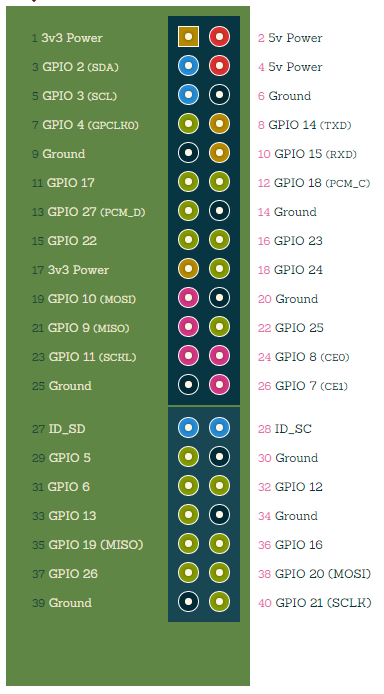
\includegraphics[width=65mm,scale=0.5]{./images/pinout.png}
%\caption{Raspberry Pi 2 Pinout \cite{pinout}.}
%\label{fig:rpi2}
%\end{center}
%\end{figure}
		\clearpage
		%!TEX root =  ../final-report.tex
\renewcommand{\lstlistingname}{Code}% Listing -> Algorithm

\chapter[Appendix B]{S-Parameter Data Acquisition System Software}
\label{appendix:software}

\section{gbin.sh}
\label{appendix:gbinsh}
\lstdefinestyle{sh}{language=bash,
  basicstyle=\ttfamily,
  literate = {\$\#}{{{\$\#}}}2,
  commentstyle=\color{red},
  keywordstyle=\color{blue},
  frame=single,
  numberstyle=\footnotesize, 
  numbers=left,
  numbersep=5pt,
  backgroundcolor=\color{white}, 
  breaklines=true}
\lstinputlisting[style=sh, caption=S-Parameter Data Acquisition Shell Script Software]{code/gbin.sh} 

\section{put2str.cs}
\label{appendix:put2str}

\definecolor{bluekeywords}{rgb}{0.13,0.13,1}
\definecolor{greencomments}{rgb}{0,0.5,0}
\definecolor{redstrings}{rgb}{0.9,0,0}

\lstdefinestyle{c}{language=[Sharp]C,
  showspaces=false,
  showtabs=false,
  breaklines=true,
  showstringspaces=false,
  breakatwhitespace=true,
  escapeinside={(*@}{@*)},
  commentstyle=\color{greencomments},
  keywordstyle=\color{bluekeywords}\bfseries,
  stringstyle=\color{redstrings},
  basicstyle=\ttfamily,
  numberstyle=\footnotesize, 
  numbers=left,
  numbersep=5pt,
  frame=single}
  
\lstinputlisting[style=c, caption=Post-Data Processing Program]{code/put2str.cs} 


\section{button.py}
\label{appendix:button}
\definecolor{keywords}{RGB}{255,0,90}
\definecolor{comments}{RGB}{0,0,113}
\definecolor{red}{RGB}{160,0,0}
\definecolor{green}{RGB}{0,150,0}
 
\lstdefinestyle{python}{language=Python, 
        basicstyle=\ttfamily\small, 
        keywordstyle=\color{keywords},
        commentstyle=\color{comments},
        stringstyle=\color{red},
        showstringspaces=false,
        identifierstyle=\color{green},
        frame=single,
        breaklines=true,
        numberstyle=\footnotesize, 
  		numbers=left,
 		numbersep=5pt,}
		
\lstinputlisting[style=python, caption=Button and LED function on Raspberry Pi 2]{code/button.py}        

\section{gbin.xml}



\lstdefinestyle{xml}{language=XML,
      showspaces=false,
      showtabs=false,
      breaklines=true,
      showstringspaces=false,
      stringstyle=\color{bluekeywords},
      keywordstyle=\color{redstrings},
      morekeywords={name, connectionString, providerName},
      commentstyle=\color{greencomments},
      frame=single,
      basicstyle=\ttfamily,
      numberstyle=\footnotesize, 
 	  numbers=left,
	  numbersep=5pt,}
      
\lstinputlisting[style=xml, caption=miniVNA PRO XML Software Configuration File]{code/gbin.xml}

\label{appendix:xml}

\section{Dropbox Setup on the Raspberry Pi 2}
\label{appendix:dropbox}

The instructions below shows how a user can setup Dropbox on the Raspberry Pi 2 and how it can be linked to their Dropbox account. Note that an Internet connection is required for this installation. For more information on the Dropbox Uploader shell script, please refer to Andrea Fabriz's Github \cite{dropbox}.

\subsection{Setup Instructions}
\begin{enumerate}
\item The Dropbox shell script can be downloaded using the following command:
\begin{verbatim}$ wget https://raw.github.com/andreafabrizi/Dropbox-Uploader/master/dropbox_uploader.sh$
\end{verbatim}
\item Permissions on the shell script will need to be changed to make it executable. This can be done by the following command:
\begin{verbatim}$ chmod +x dropbox_uploader.sh 
\end{verbatim}
\item Now Dropbox can be configured for the first time by running 
\begin{verbatim}$ ./dropbox_uploader.sh 
\end{verbatim}
\item Follow the instructions on the screen to create a new Dropbox app on your account from another web browser.  Copy the app key and app secret given by Dropbox after filling out the create a new app form to the terminal window that is running the Dropbox shell script.  
\item If the given information is correct, you will receive a oAUTH URL to enter into your web browser to verify app access to your Dropbox.
\item Dropbox on the Raspberry Pi 2 is now linked to your account. See below for Dropbox commands that can run on the Raspberry Pi 2.
\end{enumerate}

\subsection{'dropbox-uploader.sh' Commands}

$<file/folder>$ is a required parameter
\\$[file/folder]$ is an option parameter 

\begin{verbatim}./dropbox-uploader.sh upload <LOCAL_FILE/DIR ...> <REMOTE_FILE/DIR>
\end{verbatim}
\begin{verbatim}./dropbox-uploader.sh download <REMOTE_FILE/DIR> [LOCAL_FILE/DIR]
\end{verbatim}
\begin{verbatim}./dropbox-uploader.sh delete <REMOTE_FILE/DIR>
\end{verbatim}
\begin{verbatim}./dropbox-uploader.sh move <REMOTE_FILE/DIR> [REMOTE_FILE/DIR]
\end{verbatim}
\begin{verbatim}./dropbox-uploader.sh copy <REMOTE_FILE/DIR> [REMOTE_FILE/DIR]
\end{verbatim}
\begin{verbatim}./dropbox-uploader.sh mkdir <REMOTE_DIR> 
\end{verbatim}
\begin{verbatim}./dropbox-uploader.sh list <REMOTE_DIR>
\end{verbatim}
\begin{verbatim}./dropbox-uploader.sh share <REMOTE_DIR>
\end{verbatim}
\begin{verbatim}./dropbox-uploader.sh info
\end{verbatim}
\begin{verbatim}./dropbox-uploader.sh unlink
\end{verbatim}
		\clearpage
		%!TEX root =  ../final-report.tex

\chapter[Appendix C]{Raspberry Pi 2 Pinout}
\label{appendix:rpi2}

\begin{figure}[h]
\begin{center}
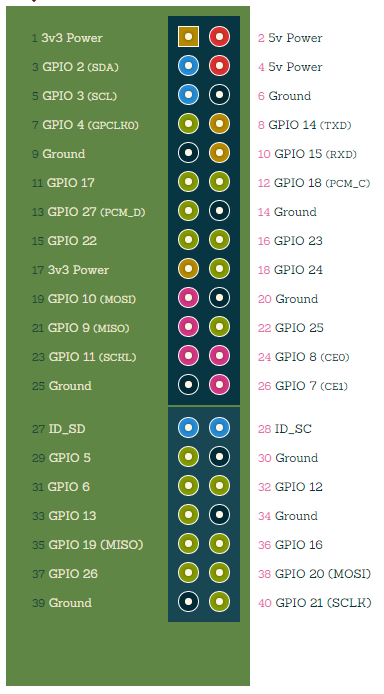
\includegraphics[width=65mm,scale=0.5]{./images/pinout.png}
\caption{Raspberry Pi 2 Pinout \cite{pinout}.}
\label{fig:rpi2}
\end{center}
\end{figure}
		\clearpage
		%!TEX root =  ../final-report.tex

\chapter[Curriculum Vitae]{Curriculum Vitae}
\label{appendix:vitae}

%%%
% Student #1
%%%
\section*{\centering \StudentNameA}
\begin{table}[htdp]
\begin{center}
\begin{tabular}{rl}
	PLACE OF BIRTH: 
		& Winnipeg, Manitoba\\
	YEAR OF BIRTH: 
		& 1990 \\
	SECONDARY EDUCATION: 
		& High School Name (2003-2008) \\
	HONOUR AND AWARDS: 
		& Governor General's Award 2003 \\
		& NSERC Undergraduate Student Researcher Award 2010 \\
%% You can other items such as extra curricular activities if you wish.		
		
\end{tabular}
\end{center}
\end{table}
%\newpage 

%%%
% Student #2
%%%
\vspace*{\stretch{2}}
\section*{\centering \StudentNameB}
\begin{table}[htdp]
\begin{center}
\begin{tabular}{rl}
	PLACE OF BIRTH: 
		& Winnipeg, Manitoba\\
	YEAR OF BIRTH: 
		& 1990 \\
	SECONDARY EDUCATION: 
		& High School Name (2003-2008) \\
	HONOUR AND AWARDS: 
		& Governor General's Award 2003 \\
		& NSERC Undergraduate Student Researcher Award 2010 \\
%% You can other items such as extra curricular activities if you wish.
\end{tabular}
\end{center}
\end{table}
\vspace*{\stretch{2}}
\newpage

%%%
% Student #3
%%%
\vspace*{\stretch{2}}
\section*{\centering \StudentNameC}
\begin{table}[htdp]
\begin{center}
\begin{tabular}{rl}
	PLACE OF BIRTH: 
		& Winnipeg, Manitoba\\
	YEAR OF BIRTH: 
		& 1990 \\
	SECONDARY EDUCATION: 
		& High School Name (2003-2008) \\
	HONOUR AND AWARDS: 
		& Governor General's Award 2003 \\
		& NSERC Undergraduate Student Researcher Award 2010 \\
%% You can other items such as extra curricular activities if you wish.
\end{tabular}
\end{center}
\end{table}
\vspace*{\stretch{2}}
%\newpage

%%%
% Student #4
%%%
\vspace*{\stretch{2}}
\section*{\centering \StudentNameD}
\begin{table}[htdp]
\begin{center}
\begin{tabular}{rl}
	PLACE OF BIRTH: 
		& Winnipeg, Manitoba\\ 
	YEAR OF BIRTH: 
		& 1990 \\ 
	SECONDARY EDUCATION: 
		& High School Name (2003-2008) \\
	HONOUR AND AWARDS: 
		& Governor General's Award 2003 \\
		& NSERC Undergraduate Student Researcher Award 2010 \\
%% You can other items such as extra curricular activities if you wish.
\end{tabular}
\end{center}
\end{table}
\vspace*{\stretch{2}}
\newpage

%%%
% Student #5
%%%
\vspace*{\stretch{2}}
\section*{\centering \StudentNameE}
\begin{table}[htdp]
\begin{center}
\begin{tabular}{rl}
	PLACE OF BIRTH: 
		& Winnipeg, Manitoba\\
	YEAR OF BIRTH: 
		& 1990 \\
	SECONDARY EDUCATION: 
		& High School Name (2003-2008) \\
	HONOUR AND AWARDS: 
		& Governor General's Award 2003 \\
		& NSERC Undergraduate Student Researcher Award 2010 \\
\end{tabular}
\end{center}
\end{table}
\vspace*{\stretch{2}}
%\newpage

%%%
% Student #6
%%%
\vspace*{\stretch{2}}
\section*{\centering \StudentNameF}
\begin{table}[htdp]
\begin{center}
\begin{tabular}{rl}
	PLACE OF BIRTH: 
		& Winnipeg, Manitoba\\
	YEAR OF BIRTH: 
		& 1990 \\
	SECONDARY EDUCATION: 
		& High School Name (2003-2008) \\
	HONOUR AND AWARDS: 
		& Governor General's Award 2003 \\
		& NSERC Undergraduate Student Researcher Award 2010 \\
%% You can other items such as extra curricular activities if you wish.
\end{tabular}
\end{center}
\end{table}
\vspace*{\stretch{2}}
%\newpage

		\clearpage
		\newpage
	\end{appendices}

%%%
% THE END
%%%
\end{document}